\section{Variable Refrigerant Flow Heat Pumps }\label{variable-refrigerant-flow-heat-pumps}

A Variable Refrigerant Flow (VRF, or Variable Refrigerant Volume) system is an air-conditioning system that varies the refrigerant flow rate using variable speed compressor(s) in the outdoor unit, and the electronic expansion valves (EEVs) located in each indoor unit. The system meets the space cooling or heating load requirements by maintaining the zone air temperature at the setpoint. The ability to control the refrigerant mass flow rate according to the cooling and/or heating load enables the use of as many as 60 or more indoor units with differing capacities in conjunction with one single outdoor unit. This unlocks the possibility of having individualized comfort control, simultaneous heating and cooling in different zones, and heat recovery from one zone to another. It may also lead to more efficient operations during part-load conditions. VRF can be divided into two common types:

\begin{itemize}
\item
  Heat Pump (HP) type: the most general type that can be used for either cooling or heating, but not simultaneously.
\item
  Heat Recovery (HR) type: can deliver simultaneous heating and cooling to different zones by transferring heat between the cooling and heating indoor units. This generally occurs in the winter season in medium-sized to large-sized commercial buildings with a substantial core such as computer rooms.
\end{itemize}

There are two alternative VRF models available in EnergyPlus to simulate the energy performance of VRF:

\begin{enumerate}
\def\labelenumi{\arabic{enumi}.}
\item
  \textbf{System Curve based Model (VRF-SysCurve)}. In this model, a number of system level curves are used to describe the VRF system performance. It uses the \emph{AirConditioner:VariableRefrigerantFlow} object to describe both the HP and HR systems.
\item
  \textbf{Physics based Model (VRF-FluidTCtrl)}. This model is able to consider the dynamics of more operational parameters and is applicable for fluid temperature control. It uses the \emph{AirConditioner:VariableRefrigerantFlow:FluidTemperatureControl:HP} object for the HP system and emph{AirConditioner:VariableRefrigerantFlow:FluidTemperatureControl:HR} for the HR system.
\end{enumerate}

\subsection{System Curve based VRF Model (VRF-SysCurve)}\label{variable-refrigerant-flow-heat-pump-model-system-curve-based-model}

\subsubsection{Overview}\label{overview-028}

This section describes the System Curve based VRF Model (VRF-SysCurve), which can address both the heat pump and heat recovery operating modes and support air-, evaporatively-, or water-cooled condenser equipment ( throughout this section, the term ``condenser'' refers to the outdoor unit where the compressor is located. )

The figure below schematically depicts the AirConditioner:VariableRefrigerantFlow (VRF AC) system. The outdoor unit is connected directly to the zone terminal units using a zone terminal unit list (ref: ZoneTerminalUnitList). The VRF AC system conditions multiple zones and is controlled by thermostats located in each zone. Zone terminal units operate to meet the zone sensible cooling or sensible heating requirements as determined by the zone thermostat schedule.

When the heat pump does \emph{\textbf{not}} operate to reclaim waste heat, the VRF AC system can only operate in either cooling \emph{or} heating mode. Based on the master thermostat priority control selection, the operating mode is determined by polling the appropriate zone(s) served by the VRF HP system. When the system is operating in cooling mode, the cooling coils will be enabled only in the terminal units where zone cooling is required. When the system is operating in heating mode, the heating coils will be enabled only in the terminal units where zone heating is required. Supply air fans will continue to operate if the zone terminal unit's fan operating mode is set to continuous fan.

When the heat pump \emph{\textbf{does}} operate to reclaim waste heat, the VRF AC system can simultaneously cool and heat multiple zones. The heat pump will select an operating mode according to the dominant load as reported by the zone thermostat(s). The calculation of the dominant load is based on the master thermostat priority control selection and may either be based on individual zone loads, the number of zones requiring cooling or heating, the master thermostat zone load, or an operating mode schedule. The heat pump will operate in cooling mode, and provide waste heat to zones with a heating load, when the dominant load among all zone terminal units is cooling. The heat pump will operate in heating mode, and absorb heat from zones with a cooling load, when the dominant load among all zone terminal units is heating.

The figure below shows the VRF AC terminal units with draw through fan placement. Blow through fan placement can also be modeled by connecting the supply air fan inlet node to the outside air mixer's mixed air node if an outdoor air mixer is used or to the zone terminal unit inlet node if an outdoor air mixer is not used. The variable refrigerant flow heat pump coordinates the operation of these components and is modeled as a type of zone equipment where the \emph{zone terminal units} are specified in a zone equipment list (Ref. ZoneHVAC: EquipmentList and ZoneHVAC:EquipmentConnections). The AirConditioner: VariableRefrigerantFlow object \emph{is not} specified in an air primary loop or a zone equipment list object.

\begin{figure}[hbtp] % fig 242
\centering
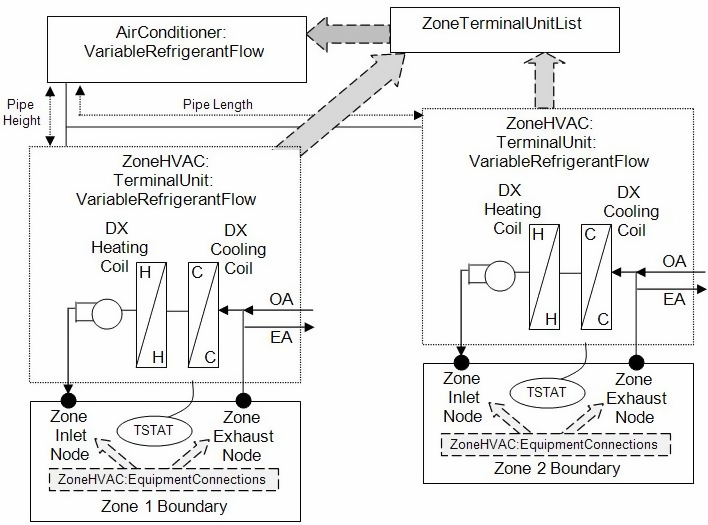
\includegraphics[width=0.9\textwidth, height=0.9\textheight, keepaspectratio=true]{media/image5315.png}
\caption{Variable Refrigerant Flow Heat Pump (draw through fan placement) \protect \label{fig:variable-refrigerant-flow-heat-pump-draw}}
\end{figure}

\begin{figure}[hbtp] % fig 243
\centering
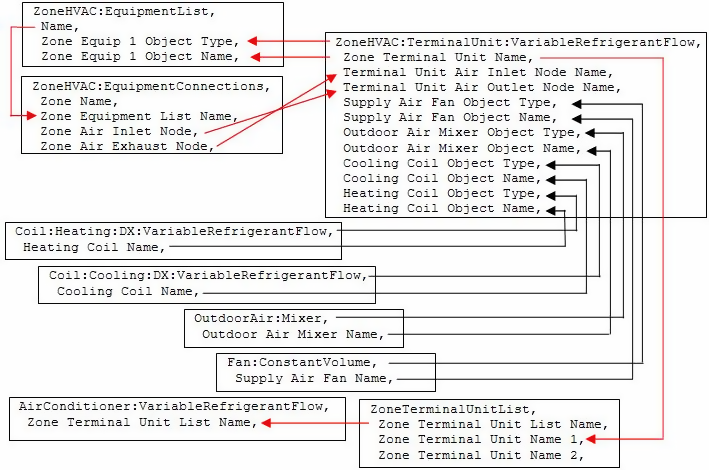
\includegraphics[width=0.9\textwidth, height=0.9\textheight, keepaspectratio=true]{media/image5316.png}
\caption{Energyplus object connections for VRF-SysCurve model \protect \label{fig:energyplus-object-connections-for-vrf}}
\end{figure}

The terminal unit is able to model supply air fan operation in two modes: cycling fan -- cycling coil (i.e., AUTO fan) and continuous fan -- cycling coil (i.e., fan ON). Fan:Simple:OnOff must be used to model AUTO fan, while Fan:Simple:OnOff or Fan:Simple:ConstVolume can be used to model fan ON.

Output variables reported by the VRF AC object include the heat pump's operating capacity (cooling or heating), electric consumption, operating COP, defrost electric consumption, part-load ratio (ratio of actual capacity to available capacity), runtime fraction (when cycling), cycling ratio (actual compressor cycling rate), crankcase heater power, and other report variables associated with an evaporative condenser. Report variables are also available to indicate the maximum available terminal unit cooling or heating capacity (i.e., when the condensers available capacity is insufficient to supply the capacity requested by all terminal units). Reporting of other variables of interest for the VRF AC (fan electric power, DX coil cooling rate, DX coil heating rate, terminal unit total cooling rate, etc.) is done by the individual system components (e.g., fan, DX cooling coil, DX heating coil, and zone terminal unit). For convenience, the total cooling and heating coil capacities (i.e., the coil loads) is also reported.

\subsubsection{Model Description}\label{model-description-015}

As described previously, the VRF AC system conditions multiple zones and is controlled by one or more zone thermostats (ZoneControl:Thermostatic). Each simulation time step, EnergyPlus performs a zone air heat balance to determine if cooling or heating is required to meet each zone's thermostat set point. When heat pump mode is selected (i.e., heat recovery is not selected), an operating mode is chosen based on the master thermostat priority control and all terminal units are operated in that specific mode. When heat recovery mode is selected, the dominant load is determined based on the master thermostat priority control and the outdoor unit operates in this mode. The indoor terminal units operate in either cooling or heating mode based on the individual coil loads. The heat pump condenser is then modeled to determine any impact the condensing unit might have on the zone terminal units (i.e., capacity limitations due to over-sized terminal units, operating limitations due to allowable operating temperature range, impacts of defrost operation, changes in performance when heat recovery mode is active, etc.). The following sections describe the performance calculations for cooling and heating.

\subsubsection{Cooling Operation}\label{cooling-operation-000}

The operating capacity of the heat pump is calculated based on the user defined input for the heat pump's rated cooling capacity, the ratio of indoor terminal unit capacity to outdoor unit capacity (combination ratio), the actual operating conditions, and whether or not the system's heat recovery mode is active. Performance correction factors are used to correct for off-design performance as follows:

\subsubsection{Cooling Combination Ratio Correction Factor}\label{cooling-combination-ratio-correction-factor}

The cooling combination ratio correction factor is defined as the total terminal unit rated cooling capacity divided by the heat pump's rated cooling capacity. The combination ratio is important when multiple terminal units (or DX coils) are attached to a single variable-speed condensing unit. If the combination ratio is less than 1, the condenser's rated capacity is assumed to be able to meet the indoor terminal unit's demand request. However, if the combination ratio is determined to be greater than 1, the maximum cooling capacity available from the heat pump's condenser may be higher than the user specified rated cooling capacity. The combination ratio capacity correction factor is based on a linear, quadratic or cubic curve and provides a multiplier \textgreater{} 1 to correct for combination ratio's greater than 1. For example, a combination ratio of 1.3 (130\%) may result in a combination ratio capacity correction factor of 1.06 (outdoor condenser can actually provide 106\% of rated capacity) . The cooling combination ratio correction factor is applied to cooling performance calculations. If the cooling combination ratio correction curve name is not specified by the user, the cooling combination ratio correction factor (CR\(_{cooling,correction}\)) in the following equation is assumed to be equal to 1.

\begin{equation}
  CR_{cooling,rated} = \frac{\sum \limits_1^n \dot{Q}_{coil(i),cooling,rated}}{\dot{Q}_{cooling,total,rated}}
\end{equation}

\begin{equation}
C{R_{cooling,correction}} = a + b\left( {C{R_{cooling,rated}}} \right) + c{\left( {C{R_{cooling,rated}}} \right)^2} + d{\left( {C{R_{cooling,rated}}} \right)^3}
\end{equation}

\begin{equation}
C{R_{cooling,correction}} = MAX\left( {1.0,C{R_{cooling,correction}}} \right)
\end{equation}

where:

\({\dot{Q}_{coil(i),cooling,rated}}\) is the rated total (sensible + latent) cooling capacity in zone \emph{i} (W)

\({\dot{Q}_{cooling,total,rated}}\) is the rated total cooling capacity of heat pump (W)

\(C{R_{cooling,correction}}\) is the Cooling Combination Ratio capacity correction factor at rated conditions (this value is reported in the eio file)

\(a - d\) are the equation coefficients for cooling combination ratio correction factor

\(C{R_{cooling,rated}}\) is the cooling combination ratio defined as the total indoor terminal unit's rated total cooling capacity divided by the rated total cooling capacity of the heat pump condenser.

The sum of the individual zone total cooling requirements is used to calculate the performance of the outdoor condensing unit. The operating capacities of the indoor cooling coils are calculated based on the indoor cooling coil's rated cooling capacity and the actual operating conditions. The operating capacity of the heat pump condenser is calculated in a similar fashion using a load-weighted average indoor wet-bulb temperature of all operating cooling coils.

\subsubsection{Cooling Capacity Ratio Modifier Function of Low Temperature}\label{cooling-capacity-ratio-modifier-function-of-low-temperature}

The heat pump's cooling capacity correction factor (function of temperature) is determined by averaging the zone cooling coil inlet air wet-bulb temperature for all operating cooling coils. A load-weighted average inlet air wet-bulb temperature is used in the calculations. The weighted average cooling coil inlet air wet-bulb temperature and the outdoor condenser entering air dry-bulb temperature are then used to calculate the temperature correction factor in cooling mode for the heat pump condenser. If the \textit{Condenser Type} is WaterCooled, then the cooling capacity curve will be function of weighted average cooling coil inlet air wet-bulb temperature and outdoor condenser entering water temperature. The actual zone air wet-bulb temperature is used to calculate the operating capacity of the individual zone cooling coils.

\begin{equation}
{\dot{Q}_{zone,total}} = \sum\limits_1^i {\dot{Q}_{zone(i)}}
\end{equation}

\begin{equation}
  T_{wb,avg} = \sum\limits_1^i {\PB{T_{wb,i}}} \PB{\frac{\dot{Q}_{zone(i)}}{\dot{Q}_{zone,total}}}
\end{equation}

The operating capacity of the heat pump is calculated using a bi-quadratic equation using a load-weighted average indoor wet-bulb temperature and outdoor dry-bulb temperature as the independent variables.

\begin{equation}
CAPF{T_{HP,cooling}} = a + b\left( {{T_{wb,avg}}} \right) + c{\left( {{T_{wb,avg}}} \right)^2} + d\left( {{T_c}} \right) + e{\left( {{T_c}} \right)^2} + f\left( {{T_{wb,avg}}} \right)\left( {{T_c}} \right)
\end{equation}

The operating capacity of the terminal unit's DX cooling coil is calculated using either a linear, quadratic, or cubic curve. If more information is available to more accurately model the DX cooling coil, a bi-quadratic curve may be used (i.e., if the performance of the DX cooling coil is also a function of outdoor dry-bulb temperature).

\begin{equation}
CAPF{T_{coil,\,cooling}} = a + b\left( {{T_{wb,i}}} \right) + c{\left( {{T_{wb,i}}} \right)^2} + d{\left( {{T_{wb,i}}} \right)^3}
\end{equation}

or

\begin{equation}
CAPF{T_{coil,cooling}} = a + b\left( {{T_{wb,i}}} \right) + c{\left( {{T_{wb,i}}} \right)^2} + d\left( {{T_c}} \right) + e{\left( {{T_c}} \right)^2} + f\left( {{T_{wb,i}}} \right)\left( {{T_c}} \right)
\end{equation}

where:

\({T_{wb,i}}\) is the wet-bulb temperature of the air entering the cooling coil in zone \emph{i} (\(^{\circ}\)C)

\({T_{wb,avg}}\) is the load-weighted average wet-bulb temperature of the air entering all operating cooling coils (\(^{\circ}\)C)

\({\dot{Q}_{zone(i)}}\) is the total (sensible + latent) cooling load in zone \emph{i} (W)

\({\dot{Q}_{zone,\,total}}\) is the total (sensible + latent) cooling load in all zones (W)

\(CAPF{T_{HP,cooling}}\) is the heat pump Cooling Capacity Ratio Modifier (function of temperature)

\(CAPF{T_{coil,cooling}}\) is the zone coil Cooling Capacity Ratio Modifier (function of temperature)

\(a - f\) are the equation coefficients for Cooling Capacity Ratio Modifier

\({T_c}\) is the temperature of the air entering an air-cooled or evaporatively-cooled condenser (\(^{\circ}\)C).

\subsubsection{Using multiple curves to define Cooling Capacity Ratio Modifier}\label{using-multiple-curves-to-define-cooling-capacity-ratio-modifier}

The cooling capacity ratio modifier determines the change in total (sensible + latent) capacity with respect to the heat pump rated cooling capacity. This modifier corrects for off-design performance and provides the operating total (sensible + latent) cooling capacity for the heat pump condenser. The performance data for VRF AC systems may be specified using a single curve object, however, if the performance data does not reflect a smooth change in performance as outdoor conditions vary, the overall performance of the system may be described using two cooling capacity ratio modifier curves (i.e., a separate curve at low and high outdoor temperatures) and a boundary curve (i.e., the curve defining the separation at specific outdoor temperatures). If the \textit{Condenser Type} is WaterCooled, the cooling capacity and EIR modifier curves may be represented using the low temperature curve input field only.

\subsubsection{Application of Dual Performance Curves}\label{application-of-dual-performance-curves}

Two additional inputs are available to more accurately model the cooling performance of a VRF AC system. The first additional input is a boundary curve which is used to distinguish differences in performance at ``low'' and ``high'' outdoor temperature regions and the second input is a cooling capacity performance curve for the ``high'' outdoor temperature region. The boundary curve is a linear, quadratic or cubic curve defining the outdoor temperature as a function of average indoor wet-bulb temperature. The cooling capacity ratio function of high temperature curve is a biquadratic curve using average indoor wet-bulb temperature and outdoor dry-bulb temperature as the two independent variables. These additional curves are used to define the performance over two separate performance regions as shown in Figure~\ref{fig:non-linear-performance-of-vrf-heat-pump-in-cooling-mode}. The red circles in the figure identify the points at which the performance changes abruptly (i.e., slopes or shapes are significantly different) and are used to create the boundary curve. The performance on either side of the boundary curve can be a smooth curve changing with outdoor condition or a flat plateau where system controls maintain a constant operating condition. This type of performance cannot be accurately simulated using a single performance curve object. For this reason, dual capacity performance curves may be used.

Note: If the cooling performance can be described using a single performance curve object, the boundary and high temperature performance curve objects are not required.

Manufacturers may also provide this information in a tabular format. In this case the data should first be graphically displayed to identify any non-linearities and to also identify where an abrupt change in performance occurs so that a boundary curve can be created.

The cooling capacity ratio boundary curve object is used to differentiate between dual cooling capacity ratio performance curves. This curve defines the outdoor temperature below which the cooling capacity ratio function of low temperature curve object is used, otherwise, the cooling capacity ratio function of high temperature curve object is used.

\begin{equation}
{T_{OA,DB}} = a + b\left( {{T_{I,WB}}} \right) + c{\left( {{T_{I,WB}}} \right)^2} + d{\left( {{T_{I,WB}}} \right)^3}
\end{equation}

where:

T\(_{OA,DB}\) is the outside air dry-bulb temperature (\(^{\circ}\)C)

a-d are the coefficients for cooling capacity ratio boundary curve object

T\(_{I,WB}\) is the weighted average indoor wet-bulb temperature (\(^{\circ}\)C).

For the performance data shown below in Figure~\ref{fig:performance-data-for-variable-refrigerant-flow-air-conditioner-model}, the boundary curve would be created by identifying the outdoor dry-bulb temperature at which the performance changed abruptly for each of the indoor wet-bulb temperature curves shown in the figure. The following example shows the data interpreted from the figure used to regress the cooling capacity ratio boundary curve coefficients. For this example, the regression coefficients were found to be: A1 = 29.87396, B1 = -0.6928, C1 = 0.01928, D1 = -0.000532.

\begin{figure}[hbtp] % table 73
\centering
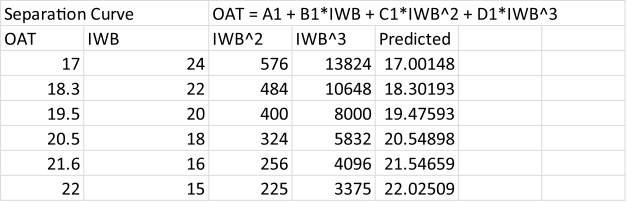
\includegraphics[width=0.9\textwidth, height=0.9\textheight, keepaspectratio=true]{media/image5339.png}
\caption{Performance Data for Variable Refrigerant Flow Air Conditioner Model \label{fig:performance-data-for-variable-refrigerant-flow-air-conditioner-model}}
\end{figure}

Although the capacity and energy performance curves each have an independent boundary curve input, in this example the same boundary curve may be used for both the capacity and energy input ratio curves. When the ``low'' and ``high'' predicted performance data do not line up at the boundary curve points, the boundary curve may have to be modified slightly to allow a smooth transition in performance from the ``low'' to ``high'' temperature region. In this case, the boundary curves for capacity and energy may be different.

\begin{figure}[hbtp] % figure 244
\centering
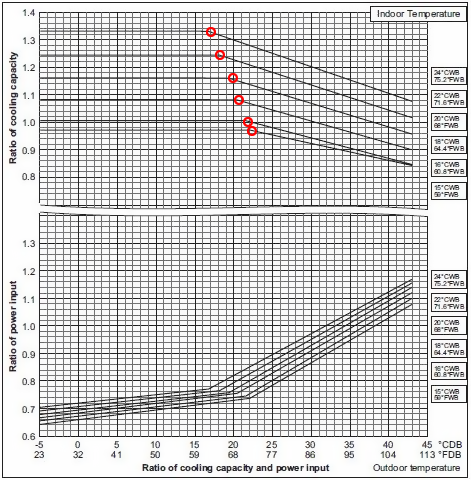
\includegraphics[width=0.9\textwidth, height=0.9\textheight, keepaspectratio=true]{media/image5340.png}
\caption{Non-Linear Performance of VRF Heat Pump in Cooling Mode \label{fig:non-linear-performance-of-vrf-heat-pump-in-cooling-mode}}
\end{figure}

A regression is then performed on the data to the left of the boundary curve to calculate the low temperature cooling performance curve coefficients. A regression is also performed on the data to the right of the boundary curve to create the high temperature cooling performance curve coefficients. The model then uses the boundary curve to determine which performance curve (low or high) to use during the simulation. For example, given a particular average indoor wet-bulb temperature, if the boundary curve object calculates an outdoor dry-bulb temperature that is above the actual outdoor dry-bulb temperature then the cooling capacity ratio function of low temperature performance curve is used to determine AC system performance for that specific simulation time step. When creating the boundary curve, be careful to make sure the low and high performance curves meet, as closely as possible, at the boundary curve points (i.e., that discontinuities do not exist or are minimized to the extent possible). Tabular data may also be used to specify performance and will usually eliminate the need for dual performance curves.

\subsubsection{Determining Cooling Coil Sensible Capacity}\label{determining-cooling-coil-sensible-capacity}

The zone terminal unit's cooling coil is controlled by a zone thermostat and must meet a zone ``sensible'' load. The cooling coil's sensible capacity is defined as the cooling coil's total capacity multiplied by the coil's sensible heat ratio (SHR) at the current operation conditions. Since the SHR of the variable refrigerant flow cooling coil changes as the inlet air wet-bulb temperature and the operating part-load ratio change, an iterative solution technique must be used to determine the coil's sensible capacity. The target solution is found when the sensible capacity of the zone cooling coil equals the zone sensible cooling load (if sufficient capacity is available). The iterative solution converges when the difference (error) between the zone sensible cooling load and the terminal unit sensible cooling capacity is within tolerance (0.001) or the terminal unit has insufficient capacity to meet the zone sensible cooling load. Refer to the description of the VRF cooling coil model for further details (ref: Variable Refrigerant Flow Cooling Coil).

\begin{equation}
  \dot{Q}_{coil(i),cooling,total} = \dot{Q}_{coil(i),cooling,rated} \left( CAPFT_{coil,cooling} \right)
\end{equation}

\begin{equation}
  PLR_i = 1
\end{equation}

\begin{equation}
  \begin{array}{l}
    Iteration~Loop~(PLR_i) \\
    ~~~~SHR_{PLR} = f \left( T_{wb,i},PLR_i,\dot{m}_i \right) \\
    ~~~~\dot{Q}_{coil(i),cooling,sensible} = \dot{Q}_{coil(i),cooling,total} \left( SHR_{PLR} \right) \left( PLR_i \right) \\
    ~~~~Error = \left( \dot{Q}_{zone(i)} - \dot{Q}_{coil(i),cooling,sensible} \right) / \dot{Q}_{zone(i)} \\
    End~Iteration~Loop
  \end{array}
\end{equation}

where:

\(\dot{Q}_{coil(i),cooling,total}\) is the zone terminal unit total (sensible + latent) cooling capacity (W), report variable ``Zone VRF Air Terminal Total Cooling Rate''

\(\dot{Q}_{coil(i),cooling,sensible}\) is the zone terminal unit sensible cooling capacity (W), report variable ``Zone VRF Air Terminal Sensible Cooling Rate''

\(PLR_i\) is the cooling coil sensible part-load ratio in zone \emph{i}

\(SHR_{PLR}\) is the cooling coil sensible heat ratio (function of PLR, inlet air wet-bulb temperature, and cooling coil inlet air mass flow rate)

\(\dot{m}_{i}\) is the cooling coil inlet air mass flow rate (m\(^3\)/s).

The terminal unit total cooling (sensible + latent) capacity is then summed to provide the total terminal unit cooling requirement. The cooling coils capacity includes the impacts of fan heat and any outdoor air provided to the zone.

\begin{equation}
  \dot{Q}_{cooling,TerminalUnits} = \sum\limits_1^i \left( \dot{Q}_{coil(i),cooling,total} \right) \left( PLR(i) \right)
\end{equation}

where \(\dot{Q}_{cooling,\,TerminalUnits}\) is the total terminal unit cooling requirement (sensible + latent) in all zones (W).

The piping correction factor is then used to adjust the total zone cooling requirement to account for piping losses in the air conditioner's refrigeration piping system.

\subsubsection{Cooling Piping Correction Factor in cooling mode}\label{cooling-piping-correction-factor-in-cooling-mode}

The cooling piping correction factor is calculated using either one or two independent variables. Both the equivalent piping length and the combination ratio are used together to determine piping losses, or the equivalent piping length itself is used. The vertical height specified by the user is also added to the result calculated by either. If a single independent variable is used, a linear, quadratic, or cubic equation is used to determine the equivalent length correction factor. If two independent variables are used, a biquadratic equation is used to determine the equivalent length correction factor. The program will automatically use the correct equation based on the performance curve type. In either case, a single coefficient adjusts the piping correction factor based on the difference in height from the highest to lowest terminal unit. Coefficients a-d (e) in the following equation(s) are inputs in the piping correction factor for length in cooling mode performance curve object. Coefficient f is a direct input to the VRF model as the piping correction factor for height in cooling mode coefficient. The equivalent piping length in cooling mode (P\(_{EQ,cooling}\)) is also a direct input in the VRF model. The cooling combination ratio (CR\(_{cooling}\)) is automatically calculated by the program. The vertical height, the difference between the highest and lowest terminal unit (e.g., 12 m higher than condenser – 3 m lower than condenser = 9 m height), is a common input for both cooling and heating. When all terminal units are above or below the outdoor unit, an average positive or negative value is used. The limits on the calculated cooling piping correction factor are 0.5 < P\(_{correction,cooling}\) < 1.

\begin{equation}
  CR_{cooling} = \frac{\sum\limits_1^n {\dot{Q}_{coil(i),cooling,rated}}}{\dot{Q}_{cooling,total,rated}}
\end{equation}

\begin{equation}
  P_{correction,cooling} = a + b \left( P_{EQ,cooling} \right) + c \left( P_{EQ,cooling} \right)^2 + d \left( P_{EQ,cooling} \right)^3 + f \left( P_H \right)
\end{equation}

or

\begin{equation}
  \begin{array}{rl}
  P_{correction,\,cooling} =& a + b \left( P_{EQ,cooling} \right) + c \left( P_{EQ,cooling} \right)^2 + d \left( CR_{cooling} \right) + e \left( CR_{cooling} \right)^2 \\
 & + f \left( P_{EQ,cooling} \right) \left( CR_{cooling} \right) + g \left( P_H \right)
  \end{array}
\end{equation}

where:

\({P_{\,correction,cooling}}\) is the Piping Correction Factor in Cooling Mode

\emph{a -- f} are equation coefficients for piping correction factor in cooling mode

\emph{g} is the user specified piping correction factor for height in cooling mode coefficient

\(P_{EQ,\,cooling}\) is the user specified equivalent piping length in cooling mode (m)

\(CR_{cooling}\) is the combination ratio in cooling mode (total rated indoor terminal unit capacity divided by the rated condenser cooling capacity) (reported to eio file)

\(P_H\) is the user specified vertical height used for piping correction factor calculation (m).

An example piping correction factor chart is shown in the following figure. The height selected for use in the equation above is selected to minimize the piping correction factor and serves to identify the worst case piping losses.

\begin{figure}[hbtp] % figure 245
\centering
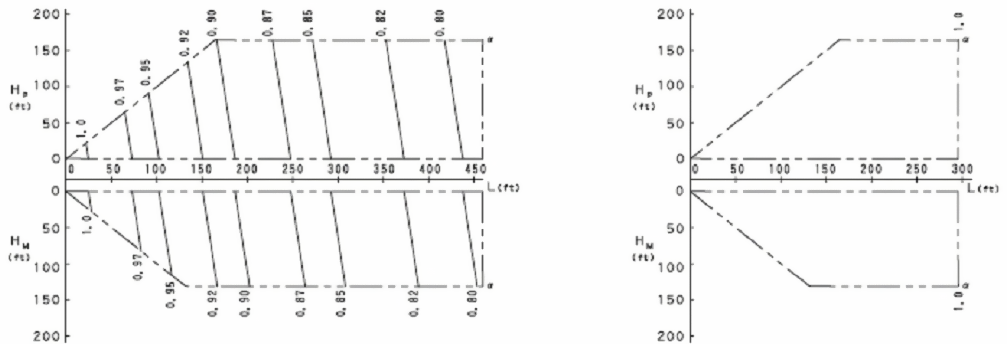
\includegraphics[width=0.9\textwidth, height=0.9\textheight, keepaspectratio=true]{media/image5358.png}
\caption{Typical Piping Factor Correction Chart \label{fig:typical-piping-factor-correction-chart}}
\end{figure}

The total demand on the heat pump condenser is then calculated as the quotient of the total terminal unit cooling capacity and the cooling piping correction factor. The piping losses are fixed throughout the simulation (i.e., these losses are not based on which terminal units are requesting refrigerant).

\begin{equation}
  \dot{Q}_{cooling,total} = \frac{\dot{Q}_{cooling,TerminalUnits}}{P_{correction,cooling}}
\end{equation}

The heat pump's total available cooling capacity is then calculated as:

\begin{equation}
  \dot{Q}_{HP,cooling,total} = \dot{Q}_{cooling,total,rated} \left( CAPFT_{HP,cooling} \right) \left( CR_{cooling,correction} \right)
\end{equation}

where:

\(\dot{Q}_{cooling,total}\) is the total heat pump condenser cooling load (W)

\(\dot{Q}_{HP,cooling,total}\) is the heat pump total available cooling capacity (W).

\subsubsection{Heat-Recovery-Cooling-Capacity-Modifier}\label{heat-recovery-cooling-capacity-modifier}

When operating in heat recovery mode, the heat pump's available cooling capacity is typically different than the available capacity when operating in cooling only mode. This modifier is used to adjust the available cooling capacity using a fraction when heat recovery is active. This fraction is based on a bi-quadratic equation with indoor and outdoor temperatures used as the independent terms.

\begin{equation}
  HRCapMod_{HP,cooling} = a + b \left( T_{ent} \right) + c \left( T_{ent} \right)^2 + d \left( T_{cond} \right) + e \left( T_{cond} \right)^2 + f \left( T_{ent} \right) \left( T_{cond} \right)
\end{equation}

This equation can be used to provide a constant fractional difference for available cooling capacity in heat recovery mode (i.e., only \emph{a} is non-zero) or a fractional term that varies with indoor and outdoor conditions. With very limited performance data available at this time, it is recommended that only the constant (a) term be used at this time. When the VRF system is not operating in heat recovery mode, this fraction is set to 1. The available cooling capacity in heat recovery mode is then:

\begin{equation}
  \dot{Q}_{HR,cooling,total} = \dot{Q}_{HP,cooling,total} \left( HRCapMod_{HP,cooling} \right)
\end{equation}

where \(\dot{Q}_{HR,cooling,total}\) = heat recovery total available cooling capacity (W).

The figure below shows VRF system laboratory data for cooling only mode (solid characters) and heat recovery mode (dotted characters). Using the limited laboratory data, the available cooling capacity fraction used to model heat recovery mode is approximately 0.91 and the cooling energy fraction is approximately 1.14. This is the only data available at this time to estimate the impact of heat recovery mode on performance. In the bi-quadratic equation, only coefficient a should be used until more complete data sets exist. Laboratory testing will eventually provide more data and better estimates of performance in heat recovery mode.

\begin{figure}[hbtp] % figure 246
\centering
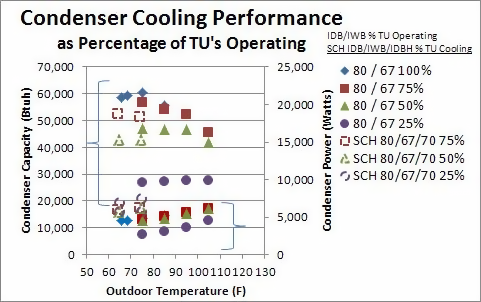
\includegraphics[width=0.9\textwidth, height=0.9\textheight, keepaspectratio=true]{media/image5366.png}
\caption{Comparison of cooling only and heat recovery mode operation \label{fig:comparison-of-cooling-only-and-heat-recovery-mode-operation}}
\end{figure}

\subsubsection{Transition from Cooling Only mode to Heat Recovery mode}\label{transition-from-cooling-only-mode-to-heat-recovery-mode}

When the VRF system transitions from cooling only operation to heat recovery operation, this transition takes some finite amount of time. During the transition period the available cooling capacity can change significantly, The following figure illustrates the transition between cooling only mode and heat recovery mode. For this test, the VRF system was turned on and allowed to reach steady-state operation. Three of the four indoor terminal units were operating in cooling mode, When the fourth terminal unit was enabled in heating mode, the transition from cooling only mode to heat recovery mode took approximately 45 minutes. During this time, the available cooling is significantly reduced and recovers over time. When the system again reaches steady-state operation, the available cooling capacity and power consumption are markedly different. Although computer models do not typically simulate this type of transitional performance, efforts to model this aspect of performance were included in the VRF AC heat recovery model. The initial heat recovery cooling capacity fraction and heat recovery cooling capacity time constant are used to model this transition period. The initial heat recovery cooling capacity fraction identifies the fraction of available heat recovery mode cooling capacity at the start of the transition period, the heat recovery cooling capacity time constant identifies the time needed to recover to 99\% of the steady-state value. This exponential model used for simulating the transition period can be turned off by setting the initial heat recovery cooling capacity fraction to 1.

\begin{figure}[hbtp] % figure 247
\centering
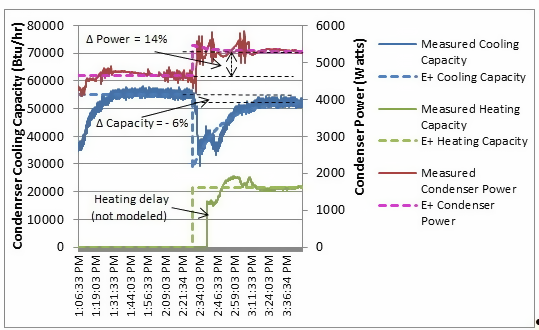
\includegraphics[width=0.9\textwidth, height=0.9\textheight, keepaspectratio=true]{media/image5367.png}
\caption{Laboratory test identifies performance changes during transition period \label{fig:laboratory-test-identifies-performance-changes-during-transition-period}}
\end{figure}

\subsubsection{Heat Recovery Cooling Capacity Fraction and Time Constant}\label{heat-recovery-cooling-capacity-fraction-and-time-constant}

When the heat pump changes operating modes (i.e., from cooling only to heat recovery mode), the transition does not happen immediately. There is a time delay, and a period of time where the available cooling capacity is well below the steady-state capacity available after the system has had time to adjust. When this type of transition is modeled, an exponential decay curve is used. At the start of the transition period, only a fraction (\(k_{cool}\)) of the steady-state capacity in heat recovery mode is available. The remaining capacity is recovered over a period of 5 time constants (t\(_{c}\)) and is modeled with the following equation. This equation was used to replicate both the cooling capacity and condenser power curves in the previous figure.

\begin{equation}
  \dot{Q}_{HR,avail,cooling} = k_{cool} \left( \dot{Q}_{HR,cooling,total} \right) + \left( 1 - k_{cool} \right) \left( \dot{Q}_{HR,cooling,total} \right) \left( 1 - e^{\left( -t / \tau_c \right)}  \right)
\end{equation}

where:

\(k_{cool}\) is the fraction of steady-state capacity at beginning of heat recovery mode

\emph{t}\(_c\) is the time constant to reach steady-state operation, 5 time constants equals 99\% of steady-state capacity (hr)

\(Q_{HR,avail,cooling}\) is the available cooling capacity in heat recovery mode (W)

\(\left( 1 - e^{\left( -t / t_{c,cool} \right)} \right)\) is the multiplier used during the transition period from cooling mode to heat recovery mode. This multiplier can be viewed using the report variable ``VRF Heat Pump Heat Recovery Status Change Multiplier'' (ref: object Output:Variable).

The operating part-load ratio of the VRF system can then be calculated:

\begin{equation}
  PLR = \frac{\dot{Q}_{cooling,total}}{\dot{Q}_{HR,avail,cooling}}
\end{equation}

where \(PLR\) is the heat pump part-load ratio, report variable ``VRF Heat Pump Part Load Ratio''.

Note: for calculation purposes \(\dot{Q}_{HR,avail,cooling}\) is equivalent to \(\dot{Q}_{HR,cooling,total}\) when heat recovery mode is not active.

The heat pump total available cooling capacity must be greater than or equal to the total cooling capacity requested by the zone terminal units. When the total operating capacity of all terminal unit's will be greater than the available operating capacity of the heat pump condenser, one or more of the terminal unit's operating capacity must be reduced to the point where the sum of the indoor terminal unit demand request plus piping losses is equal to the total available cooling capacity of the outdoor condenser. At this point, the part-load ratio of the heat pump condenser will be equal to 1.

A maximum terminal unit cooling capacity limit is used to restrict the cooling capacity of each indoor terminal unit. The capacity limit is equivalent to a maximum allowed operating capacity for all zone terminal units. This limit is used to conserve energy between multiple indoor terminal units and a single outdoor condensing unit. Assuming no terminal unit can provide more capacity than can be delivered by the outdoor condenser, the terminal unit total cooling capacity calculation previously discussed is revised as follows:

\begin{equation}
  \dot{Q}_{coil(i),\,cooling} = \sum\limits_1^i MIN \left( \left( \dot{Q}_{coil(i),cooling,total} \right) \left( PLR(i) \right),CoolingCapacityLimit \right)
\end{equation}

where \(CoolingCapacityLimit(CL_{cooling})\) is the report variable (ref: Output:Variable) describing the ``VRF Heat Pump Maximum Capacity Cooling Rate'' (W).

When multiple terminal units are operating, the terminal units near their maximum capacity are more likely to be capacity limited than those terminal units operating well below their available capacity. The assumption here is that terminal units that are not capacity limited can provide more refrigerant to meet the same load. When the model finds that there is no terminal unit capacity limit, this variable will report 1E+20 indicating that no limit exists.  The figure below demonstrates the application of the capacity limit factor for the case where all indoor terminal units are operating at different capacities. A solution is reached when the sum of the indoor terminal unit's cooling capacities (accounting for piping losses) is equal to the heat pump condenser's available cooling capacity.

\begin{figure}[hbtp] % figure 248
\centering
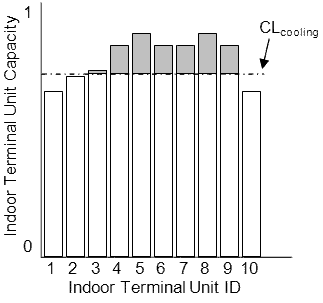
\includegraphics[width=0.9\textwidth, height=0.9\textheight, keepaspectratio=true]{media/image5376.png}
\caption{Example of Cooling Capacity Limit \label{fig:example-of-cooling-capacity-limit}}
\end{figure}

When the heat pump's part-load ratio is less than 1 (i.e., the total capacity of all terminal unit's is less than the actual operating capacity of the heat pump condenser), the heat pump's part-load ratio is compared to the minimum heat pump part-load ratio. If the heat pump's part-load ratio is less than the minimum heat pump part-load ratio, the heat pump will cycle on and off to meet the cooling load. A correction factor is used to account for startup losses of the compression system.

\textbf{Cooling Part-Load Fraction Correlation (function of cycling ratio)}

The cooling part-load fraction correlation (function of heat pump cycling ratio) is a linear, quadratic or cubic curve with the independent variable being cycling ratio (part-load ratio / minimum part-load ratio). The output of this curve is used in combination with the rated EIR and EIR modifier curves to give the ``effective'' EIR for a given simulation time step.

\begin{equation}
  CyclingRatioFrac = a + b \left( CyclingRatio \right) + c \left( CyclingRatio \right)^2 + d \left( CyclingRatio \right)^3
\end{equation}

where:

\begin{equation}
  CyclingRatio = \frac{PLR}{PLR_{min}}
\end{equation}

a-c (d) are the coefficients for the quadratic (cubic) cycling ratio correlation curve equation.

The cycling ratio can be viewed using the report variable ``VRF Heat Pump Cycling Ratio'' (ref: Output:Variable).

The cooling part-load ratio correlation should be normalized to a value of 1.0 when the cycling ratio equals 1.0 (i.e., no efficiency losses when the heat pump runs continuously [PLR \(\geq\) PLR\(_{min}\)] for the simulation time step). For cycling ratio values between 0 and 1 (0 \(\leq\) CyclingRatio < 1), the following rules apply:

\(CyclingRatioFrac \geq 0.7\) and \(CyclingRatioFrac \geq CyclingRatio\)

If CyclingRatioFrac < 0.7 a warning message is issued, the program resets the CyclingRatioFrac value to 0.7, and the simulation proceeds. The runtime fraction of the heat pump is defined as CyclingRatio/CyclingRatioFrac. If CyclingRatioFrac < CyclingRatio, the runtime fraction will exceed 1. In this case a warning message is issued and the runtime fraction of the heat pump is limited to 1.0.

\begin{equation}
  Heat~Pump~Runtime~Fraction~(HPRTF) = \frac{CyclingRatio}{CyclingRatioFrac}
\end{equation}

The heat pump runtime fraction can be viewed using the report variable ``VRF Heat Pump Runtime Fraction'' (ref: Output:Variable).

Since manufacturers data do not typically provide information defining the cycling losses of VRF AC systems, a typical part-load fraction correlation for a conventional DX refrigeration system (e.g., residential or small commercial unit) may be substituted here as:

\begin{equation}
  CyclingRatioFrac = 0.85 + 0.15(CyclingRatio)
\end{equation}

The electrical power consumed by the heat pump condenser is then calculated based on the heat pump's rated electric power consumption (including condenser fan power), the actual operating conditions, and the cycling ratio of the refrigeration system. Performance correction factors are used here to correct for off-design performance as follows:

\subsubsection{Cooling Energy Input Ratio Modifier Function of Low Temperature}\label{cooling-energy-input-ratio-modifier-function-of-low-temperature}

As described previously (Ref. Application of Dual Performance Curves), the cooling energy input ratio modifier curve can either be applied as a single curve object as shown below, or applied using dual performance curve objects. If the \textit{Condenser Type} is WaterCooled, then the cooling energy input ratio modifier curve will be function of weighted average indoor air wet-bulb temperature and outdoor condenser entering water temperature. The equation form used for a single or dual performance curve application is shown here.

\begin{equation}
  EIRFT_{cooling} = a + b \left( T_{wb,avg} \right) + c \left( T_{wb,avg} \right)^2 + d \left( T_c \right) + e \left( T_c \right)^2 + f \left( T_{wb,avg} \right) \left( T_c \right)
\end{equation}

where \(EIRFT_{cooling}\) is the cooling energy input ratio modifier (function of temperature).

\subsubsection{Cooling Energy Input Ratio Modifier Function of Part-Load Ratio}\label{cooling-energy-input-ratio-modifier-function-of-part-load-ratio}

The cooling energy input ratio calculation is based on 2 EIR curves. One is used when the heat pump part-load ratio is less than or equal to 1, and a second curve is used to describe the variation of cooling energy input ratio when the part-load ratio is greater than 1. The part-load ratio curve when PLR>1 is not a required input and when not used, the energy use is assumed to be constant when PLR > 1.

\begin{equation}
  \begin{array}{l}
  IF\left( {PLR \leq 1} \right)THEN \\
  ~~~~EIRFPLR_{cooling} = a + b \left( PLR \right) + c \left( PLR \right)^2 + d \left( PLR \right)^3 \\
  ELSE \\
  ~~~~EIRFPLR_{cooling} = e + f \left( PLR \right) + g \left( PLR \right)^2 + h \left( PLR \right)^3
  \end{array}
\end{equation}

where:

\(EIRFPLR_{cooling}\) is the cooling energy input ratio correction factor (function of part-load ratio)

a-d are the coefficient for cooling energy input ratio correlation when part-load ratio \(\leq\) 1

e-h are the coefficient for cooling energy input ratio correlation when part-load ratio > 1.

The total power consumed by the heat pump condenser in cooling mode is based on the user specified coefficient of performance (COP) and calculated as:

\begin{equation}
  CoolingPower = \left( \frac{\dot{Q}_{cooling,total,rated} CAPFT_{cooling}}{COP_{cooling,reference}} \right) \left( EIRFT_{cooling} \right) \left( EIRFPLR_{cooling} \right) \left( HPRTF \right)
\end{equation}

The cooling COP is then calculated as the ratio of the outdoor unit cooling capacity divided by the total electric consumption rate of all components associated with the outdoor unit. Although included in the equiation, defrost power is typically 0 during cooling mode operation.

\begin{equation}
  COP_{cooling} = \frac{\dot{Q}_{cooling,total}}{CoolingPower + P_{CrankCaseHeater} + P_{EvapCoolerPower} + P_{defrost}}
\end{equation}

where:

COP\(_{cooling}\) is the operating coefficient of performance, report variable ``VRF Heat Pump Cooling COP''

CoolingPower is the operating electric consumption rate (W), report variable ``VRF Heat Pump Cooling Electric Power''

P\(_{CrankcaseHeater}\) is the report variable for electric consumption rate of crankcase heater (W)

P\(_{EvapCoolerPump}\) is the report variable for electric consumption rate of evaporatively-cooled condenser water pump (W)

\({P_{defrost}}\) is the report variable for average defrost power for the simulation time step (W).

When operating in heat recovery mode, equations similar to those used for available cooling capacity are used to model heating electric consumption rate.

\begin{equation}
  HREIRMod_{HP,cooling} = a + b \left( T_{ent} \right) + c \left( T_{ent} \right)^2 + d \left( T_{cond} \right) + e \left( T_{cond} \right)^2 + f \left( T_{ent} \right) \left( T_{cond} \right)
\end{equation}

This equation can be used to provide a constant fractional difference for cooling electric consumption rate in heat recovery mode (i.e., only \emph{a} is non-zero) or a fractional term that varies with indoor and outdoor conditions. With very limited performance data available at this time, it is recommended that only the constant (a) term be used at this time. When the VRF system is not operating in heat recovery mode, this fraction is set to 1. The cooling electric consumption rate in heat recovery mode is then:

\begin{equation}
  CoolingPower_{HR} = CoolingPower \left( HREIRMod_{HP,\,cooling} \right)
\end{equation}

\begin{equation}
  Power_{HR} = k_{EIR,\,cool} \left( CoolingPower_{HR} \right) + \left( 1 - k_{EIR,\,cool} \right) \left( CoolingPower_{HR} \right) \left( 1 - e^{\left( -t / \tau_{c,\,EIR,\,cool} \right)} \right)
\end{equation}

where:

\(k_{EIR,cool}\) is the fraction of steady-state cooling electric consumption rate at beginning of heat recovery mode

\(\tau_{c,EIR,cool}\) is the time constant to reach steady-state operation, 5 time constants equals 99\% of steady-state capacity (hr)

\(CoolingPower_{HR}\) is the cooling electric consumption rate in heat recovery mode (W)

\(\left( 1 - e^{\left( -t / \tau_{c,EIR,cool} \right)} \right)\) is the multiplier used during the transition period from cooling mode to heat recovery mode. This multiplier can be viewed using the report variable ``VRF Heat Pump Heat Recovery Status Change Multiplier'' (ref: Output:Variable).

\subsubsection{Heating Operation}\label{heating-operation-201605050924}

Calculations of the heat pump's heating performance is nearly identical to the calculations described above for cooling operation.

The sum of the individual zone total heating requirements are used to calculate the performance of the outdoor condensing unit. The operating capacity of the indoor heating coils are calculated based on the indoor heating coil's nominal heating capacity and the actual operating conditions. A capacity correction factor is used to correct for off-design performance as follows:

\textbf{Heating Combination Ratio Correction Factor (function of capacity ratio)}

The heating combination ratio correction factor is defined as the total terminal unit rated heating capacity divided by the heat pump's rated heating capacity. In some instances, the cooling combination ratio may be used to define the correction factor used to modify the heat pump's rated heating capacity and is manufacturer specific. The combination ratio is important when multiple terminal units (or DX coils) are attached to a single variable-speed condensing unit. If the combination ratio is less than 1, the condenser has sufficient capacity to meet the indoor terminal unit's capacity request. However, if the combination ratio is determined to be greater than 1, the maximum heating capacity available from the heat pump's condenser may be higher than the user specified rated heating capacity. The combination ratio capacity correction factor is based on a linear, quadratic or cubic curve and provides a multiplier > 1 to correct for combination ratio's greater than 1. For example, a combination ratio of 1.3 (130\%) may result in a combination ratio capacity correction factor of 1.06 (outdoor condenser can actually provide 106\% of rated capacity) . The heating combination ratio correction factor is applied to heating performance calculations. If the heating combination ratio correction curve name is not specified by the user, the heating combination ratio correction factor (CR\(_{heating,correction}\)) in the following equation is assumed to be equal to 1.

\begin{equation}
  CR_{heating} = \frac{\sum\limits_1^n \dot{Q}_{coil(i),heating,rated}}{\dot{Q}_{heating,total,rated}}
\end{equation}

\begin{equation}
  CR_{heating,correction} = a + b \left( CR_{heating} \right) + c \left( CR_{heating} \right)^2 + d \left( CR_{heating} \right)^3
\end{equation}

\begin{equation}
  CR_{heating,correction} = MAX \left( 1.0,\,CR_{heating,correction} \right)
\end{equation}

where:

\(\dot{Q}_{coil(i),heating,rated}\) is the rated total heating capacity in zone \emph{i} (W)

\(\dot{Q}_{heating,total,rated}\) is the rated total heating capacity of heat pump (W)

\(CR_{heating,correction}\) is the heating Combination Ratio capacity correction factor at rated conditions

\(a - d\) are the cubic equation coefficients for heating combination ratio correction factor

\(CR_{heating}\) is the combination ratio in heating mode (total rated indoor terminal unit capacity divided by the rated condenser heating capacity) (reported to eio file).

\subsubsection{Heating Capacity Ratio Modifier (function of temperature)}\label{heating-capacity-ratio-modifier-function-of-temperature}

As described previously (Ref. Application of Dual Performance Curves), the heating capacity ratio modifier curve can either be applied as a single curve object as shown below, or applied using dual performance curve objects. The single curve object application is described here.

The heat pump's heating capacity ratio modifier (function of temperature) is determined by averaging the zone heating coil inlet air dry-bulb temperature for all operating heating coils. A zone load-weighted average is used when calculating the performance of the heat pump condenser. This weighted-average heating coil inlet air dry-bulb temperature and the outdoor condenser entering air wet-bulb temperature are then used to calculate the heat pump's temperature correction factor in heating mode.

Note that some manufacturers do not provide performance data as a function of outdoor wet-bulb temperature. In this case, substituting outdoor dry-bulb temperature is permitted and the Heating Performance Curve Outdoor Temperature Type input should be specified as DryBulbTemperature. This also means that performance curve coefficients for both capacity (CAPFT) and energy (EIRFT) should be calculated using indoor and outdoor dry-bulb temperature.

\begin{equation}
  T_{db,avg} = \sum\limits_1^i \left( T_{db,i} \right) \left( \frac{\dot{Q}_{zone(i)}}{\dot{Q}_{zone,\,total}} \right)
\end{equation}

\begin{equation}
  CAPFT_{HP,heating} = a + b \left( T_{db,avg} \right) + c \left( T_{db,avg} \right)^2 + d \left( T_c \right) + e \left( T_c \right)^2 + f \left( T_{db,avg} \right) \left( T_c \right)
\end{equation}

\begin{equation}
  CAPFT_{coil,heating} = a + b \left( T_{db,i} \right) + c \left( T_{db,i} \right)^2 + d \left( T_c \right) + e \left( T_c \right)^2 + f \left( T_{db,i} \right) \left( T_c \right)
\end{equation}

where:

\(T_{db,i}\) is the dry-bulb temperature of the air entering the heating coil in zone \emph{i} (\(^{\circ}\)C

\(T_{db,avg}\) is the weighted-average dry-bulb temperature of the air entering all operating heating coils (\(^{\circ}\)C

\(CAPFT_{heating}\) is the heating Capacity Correction Factor (function of temperature)

\(a - f\) are the bi-quadratic equation coefficients

\(T_c\) is the wet-bulb temperature of the air entering an air-cooled condenser (\(^{\circ}\)C.

The total terminal unit heating capacity required is the simple sum of the terminal unit capacity. If the heat pump is off or there is no zone heating requirement, the terminal unit total heating requirement will be zero. The heating coils capacity includes the impacts of fan heat and any outdoor air provided to the zone.

\begin{equation}
  \dot{Q}_{heating,TerminalUnits} = \sum\limits_1^i \left( \dot{Q}_{coil(i),heating,total} \right) \left( PLR(i) \right)
\end{equation}

where:

\(\dot{Q}_{heating,TerminalUnits}\) is the heat pump's outdoor condenser total zone heating requirement (W)

\(\dot{Q}_{coil(i),heating,total}\) is the zone terminal unit total heating capacity (W), report variable ``Zone VRF Air Terminal Total Heating Rate''.

The piping correction factor is then used to adjust the zone heating requirement to account for piping losses in the AC refrigeration system.

\subsubsection{Piping Correction Factor in heating mode}\label{piping-correction-factor-in-heating-mode}

The piping correction factor in heating mode is calculated based on the length of the farthest terminal unit and the difference in height from the highest to lowest terminal unit. The piping losses are fixed throughout the simulation (i.e., these losses are not based on which terminal units are requesting refrigerant). Coefficients a-f in the following equations are inputs in the piping correction factor for length in heating mode curve object. The curve may use either one or two independent variables. Coefficient g is a direct input to the VRF model as piping correction factor for height in heating mode coefficient. The equivalent piping length in heating mode (P\(_{EQ,heating}\)) is also a direct input in the VRF model. The vertical height (P\(_H\)), the difference between the highest and lowest terminal unit (e.g., 12 m higher than condenser – 3 m lower than condenser = 9 m height), is a common input for both cooling and heating.

\begin{equation}
  P_{correction,heating} = a + b \left( P_{EQ,heating} \right) + c \left( P_{EQ,heating} \right)^2 + d \left( P_{EQ,heating} \right)^3 + g \left( P_H \right)
\end{equation}

or

\begin{equation}
\begin{array}{rl}
{P_{correction,heating}} =& a + b \left( P_{EQ,heating} \right) + c \left( P_{EQ,heating} \right)^2 + d \left( CR_{heating} \right) + e \left( CR_{heating} \right)^2 \\
 & + f \left( P_{EQ,heating} \right) \left( CR_{heating} \right) + g \left( P_H \right)
\end{array}
\end{equation}

where:

\(P_{correction,heating}\) is the piping correction factor in heating mode

\emph{a-f} are the equation coefficients for piping correction factor in heating mode

\emph{g} is the user specified piping correction factor for height in heating mode coefficient

\(P_{EQ,heating}\) is the equivalent piping length for heating specified by the user (m)

\(P_H\) is the user specified vertical height used for piping correction factor (m).

The heat pump's total available heating capacity is then determined using the previously described modifiers.

\begin{equation}
  \dot{Q}_{HP,cooling,total} = \dot{Q}_{cooling,total,rated} \left( CAPFT_{HP,cooling} \right) \left( CR_{cooling,correction} \right)
\end{equation}

\subsubsection{Heat Recovery Heating Capacity Modifier}\label{heat-recovery-heating-capacity-modifier}

When operating in heat recovery mode, the heat pump's available heating capacity is typically different than the available capacity when operating in heating only mode. This modifier is used to adjust the available heating capacity using a fraction when heat recovery is active. This fraction is based on a bi-quadratic equation with indoor and outdoor temperatures used as the independent terms.

\begin{equation}
HRCapMod_{HP,heating} = a + b \left( T_{ent} \right) + c \left( T_{ent} \right)^2 + d \left( T_{cond} \right) + e \left( T_{cond} \right)^2 + f \left( T_{ent} \right) \left( T_{cond} \right)
\end{equation}

This equation can be used to provide a constant fractional difference for available heating capacity in heat recovery mode (i.e., only \emph{a} is non-zero) or a fractional term that varies with indoor and outdoor conditions. With very limited performance data available at this time, it is recommended that only the constant (a) term be used at this time. The available heating capacity in heat recovery mode is then:

\begin{equation}
  \dot{Q}_{HR,heating,total} = \dot{Q}_{HP,heating,total} \left( HRCapMod_{HP,heating} \right)
\end{equation}

\subsubsection{Transition from Heating Only mode to Heat Recovery mode}\label{transition-from-heating-only-mode-to-heat-recovery-mode}

When the VRF system transitions from heating only operation to heat recovery operation, this transition takes some finite amount of time. During the transition period the available heating capacity can change significantly, As described for the transition from cooling only operating to heat recovery mode, the initial heat recovery heating capacity fraction and heat recovery heating capacity time constant are used to model the transition from heating only mode to heat recovery mode. The initial heat recovery heating capacity fraction identifies the fraction of available heat recovery mode heating capacity at the start of the transition period, the heat recovery heating capacity time constant identifies the time needed to recover to 99\% of the steady-state value. This exponential model used for modeling the transition period can be turned off by setting the initial heat recovery heating capacity fraction to 1.0.

\subsubsection{Heat Recovery Heating Capacity Fraction and Time Constant}\label{heat-recovery-heating-capacity-fraction-and-time-constant}

When the heat pump changes operating modes (i.e., from heating only to heat recovery mode), the transition does not happen immediately. There is a time delay, and a period of time where the available heating capacity is different from the steady-state capacity available after the system has had time to adjust. When this type of transition is modeled, an exponential decay curve is used. At the start of the transition period, only a fraction (\(k_{heat}\)) of the steady-state capacity in heat recovery mode is available. The remaining capacity is recovered over a period of 5 time constants (\(t_{c,heat}\)) and is modeled with the following equation. This equation was used to replicate both the cooling capacity and condenser power curves in the previous figure.

\begin{equation}
  \dot{Q}_{HR,avail,heating} = k_{heat} \left( \dot{Q}_{HR,heating,total} \right) + \left( 1 - k_{heat} \right) \left( \dot{Q}_{HR,heating,total} \right) \left( 1 - e^{\left( -t / \tau_{c,heat} \right)} \right)
\end{equation}

where:

\(k_{heat}\) is the fraction of steady-state heating capacity at beginning of heat recovery mode

\(\tau_{c,heat}\) is the time constant to reach steady-state operation, 5 time constants equals 99\% of steady-state capacity (hr)

\(Q_{HR,avail,heating}\) is the available heating capacity in heat recovery mode (W)

\(\left( 1 - e^{\left( -t / \tau_{c,heat} \right)} \right)\) is the multiplier used during the transition period from heating mode to heat recovery mode. This multiplier can be viewed using the report variable ``VRF Heat Pump Heat Recovery Status Change Multiplier'' (ref: Output:Variable).

\subsubsection{Defrost Energy Input Ratio Modifier (function of temperature)}\label{defrost-energy-input-ratio-modifier-function-of-temperature}

The defrost energy input ratio (EIR) modifier curve (function of temperature) is a bi-quadratic curve with two independent variables: heating coil average entering air wet-bulb temperature and outdoor air dry-bulb temperature. The output of this curve is multiplied by the heating coil capacity, the fractional defrost time period and the runtime fraction of the heating coil to give the defrost power at the specific temperatures at which the coil is operating. The use of outdoor wet-bulb temperature is explicit in this curve object and the defrost equation below and is independent of the selection for Heating Performance Curve Outdoor Temperature Type.

\begin{equation}
  DefrostEIRTempModFac = a + b\left( {{T_{wb,avg}}} \right) + c{\left( {{T_{wb,avg}}} \right)^2} + d\left( {{T_c}} \right) + e{\left( {{T_c}} \right)^2} + f\left( {{T_{wb,avg}}} \right)\left( {{T_c}} \right)
\end{equation}

The heat pump condenser's total heating load is then calculated as the quotient of the total terminal unit capacity and the piping correction factor. Additional load due to defrost is also included (see following section).

\begin{equation}
  \dot{Q}_{heating,total} = \left( \frac{\dot{Q}_{heating,TerminalUnits}}{P_{correction,heating}} \right) + \dot{Q}_{defrost}
\end{equation}

The heat pump's total (gross) heating capacity is then calculated based on the capacity correction factor as a function of temperatures. The impact of defrost on total heat pump heating capacity is also accounted for (see following section). The part-load ratio of the heat pump condenser can then be calculated.

\begin{equation}
  \dot{Q}_{HP,total} = \dot{Q}_{total,rated} \left( CAPFT_{HP,heating} \right) \left( CR_{heating,correction} \right) \left( HCAP_{defrost} \right)
\end{equation}

\begin{equation}
  PLR = \frac{\dot{Q}_{heating,total}}{\dot{Q}_{HP,total}}
\end{equation}

where:

\(\dot{Q}_{HP,total}\) is the heat pump total available heating capacity (W)

\(PLR\) is the heat pump part-load ratio

\(HCAP_{defrost}\) is the heating capacity correction factor for defrost mode.

As described for cooling operation, the available heating capacity of the heat pump is compared to the requested heating capacity of all indoor terminal units. If the requested heating capacity of all indoor terminal units is greater than the available heating capacity of the heat pump, one or more of the indoor terminal unit's capacity is limited such that the sum of the zone terminal unit heating demand plus piping losses is equal to the available heat pump heating capacity (including the impact due to defrost).

The electrical power consumed by the heat pump condenser is calculated based on the heat pump's nominal electric power consumption in heating mode and the actual operating conditions. A performance correction factor is used to correct for off-design performance as follows:

\emph{\textbf{Heating Part-Load Fraction Correlation (function of heat pump cycling ratio)}}

The part-load fraction correlation (function of heat pump cycling ratio) is a linear, quadratic or a cubic curve with the independent variable being cycling ratio (part-load ratio / minimum part-load ratio). The output of this curve is used in combination with the rated EIR and EIR modifier curves to give the ``effective'' EIR for a given simulation time step. The cycling ratio correlation accounts for startup losses of the heat pump's compression system.

\begin{equation}
  CyclingRatioFrac = a + b \left( CyclingRatio \right) + c \left( CyclingRatio \right)^2
\end{equation}

or

\begin{equation}
  CyclingRatioFrac = a + b \left( CyclingRatio \right) + c \left( CyclingRatio \right)^2 + d \left( CyclingRatio \right)^3
\end{equation}

where

\begin{equation}
  CyclingRatio = \frac{PLR}{PLR_{\min }}
\end{equation}

The cycling ratio can be viewed using the report variable ``VRF Heat Pump Cycling Ratio'' (ref: Output:Variable).

The cycling ratio correlation should be normalized to a value of 1.0 when the cycling ratio equals 1.0 (i.e., no efficiency losses when the compressor(s) run continuously for the simulation time step). For cycling ratio values between 0 and 1 (0 \(\leq\) CyclingRatio < 1), the following rules apply:

\(CyclingRatioFrac \geq 0.7\)   and   \(CyclingRatioFrac \geq CyclingRatio\)

If CyclingRatioFrac < 0.7 a warning message is issued, the program resets the CyclingRatioFrac value to 0.7, and the simulation proceeds. The runtime fraction of the heat pump is defined as CyclingRatio/CyclingRatioFrac. If CyclingRatioFrac < CyclingRatio, then a warning message is issued and the runtime fraction of the heat pump is limited to 1.0.

\begin{equation}
  Heat~Pump~Runtime~Fraction \left( HPRTF \right) = \frac{CyclingRatio}{CyclingRatioFrac}
\end{equation}

The heat pump runtime fraction can be viewed using the report variable ``VRF Heat Pump Runtime Fraction'' (ref: Output:Variable).

Since manufacturers data do not typically provide information defining the cycling losses of VRF AC systems, a typical part-load fraction correlation for a conventional DX refrigeration system (e.g., residential or small commercial unit) may be substituted here as:

\begin{equation}
  CyclingRatioFrac = 0.85 + 0.15(CyclingRatio)
\end{equation}

\emph{\textbf{Heating Energy Input Ratio Modifier (function of temperature)}}

As described previously (Ref. Application of Dual Performance Curves), the heating energy input ratio modifier curve can either be applied as a single curve object as shown below, or applied using dual performance curve objects. The single curve object application is discussed here.

\begin{equation}
  EIRFT_{heating} = a + b \left( T_{db,avg} \right) + c \left( T_{db,avg} \right)^2 + d \left( T_c \right) + e \left( T_c \right)^2 + f \left( T_{db,avg} \right) \left( T_c \right)
\end{equation}

where \(EIRFT_{heating}\) = heating energy input ratio correction factor (function of temperature) (0-1).

\emph{\textbf{Heating Energy Input Ratio Modifier (function of part-load ratio)}}

\begin{equation}
  \begin{array}{l}
    IF \left( PLR \leq 1 \right) THEN \\
    ~~~~EIRFPLR_{heating} = a + b \left( PLR \right) + c \left( PLR \right)^2 + d \left( PLR \right)^3 \\
    ELSE \\
    ~~~~EIRFPLR_{heating} = e + f \left( PLR \right) + g \left( PLR \right)^2 + h \left( PLR \right)^3
  \end{array}
\end{equation}

where:

\(EIRFPLR_{heating}\) is the heating energy input ratio modifier (function of part-load ratio)

a-d are the coefficients for the heating energy input ratio modifier when part-load ratio \(\leq\) 1

e-h are the coefficients for the heating energy input ratio modifier when part-load ratio > 1

The total power consumed by the heat pump condenser in heating mode is then calculated. A correction for power consumed due to defrost is also included (see following section).

The total power consumed by the heat pump condenser in heating mode is based on the user specified coefficient of performance (COP). A correction for power consumed due to defrost is also included (see following section).

\begin{equation}
\begin{array}{rl}
  HeatingPower =& \left( \frac{\dot{Q}_{heating,\,total,\,rated} CAPFT_{heating}}{COP_{heating,reference}} \right) \left( EIRFT_{heating} \right) \left( EIRFPLR_{heating} \right) \\
  & * \left( HPRTF \right) \left( EIR_{defrost} \right)
\end{array}
\end{equation}

The heating COP is then calculated as the ratio of the outdoor unit heating capacity divided by the total electric consumption rate of all components associated with the outdoor unit. Evaporatively-cooled condenser pump power is typically 0 during heating mode operation.

\begin{equation}
  COP_{heating} = \dot{Q}_{heating,total} / \left( HeatingPower + P_{CrankcaseHeater} + P_{EvapCoolerPower} + P_{defrost} \right)
\end{equation}

where:

COP\(_{heating}\) is the operating coefficient of performance, report variable ``VRF Heat Pump Heating COP''

HeatingPower is the operating electric consumption rate (W), report variable ``VRF Heat Pump Heating Electric Power''.

When operating in heat recovery mode, equations similar to those used for available heating capacity are used to model operating power.

\begin{equation}
  HREIRMod_{HP,heating} = a + b \left( T_{ent} \right) + c \left( T_{ent} \right)^2 + d \left( T_{cond} \right) + e \left( T_{cond} \right)^2 + f \left( T_{ent} \right) \left( T_{cond} \right)
\end{equation}

This equation can be used to provide a constant fractional difference for heating electric consumption rate in heat recovery mode (i.e., only *a* is non-zero) or a fractional term that varies with indoor and outdoor conditions. With very limited performance data available at this time, it is recommended that only the constant (a) term be used at this time. When the VRF system is not operating in heat recovery mode, this fraction is set to 1.The available heating electric consumption rate in heat recovery mode is then calculated as:

\begin{equation}
  HeatingPower_{HR} = HeatingPower \left( HREIRMod_{HP,heating} \right)
\end{equation}

\begin{equation}
  Power_{HR} = k_{EIR,heat} \left( HeatingPower_{HR} \right) + \left( 1 - k_{EIR,heat} \right) \left( HeatingPower_{HR} \right) \left( 1 - e^{\left( -t / \tau_{c,EIR,heat} \right)} \right)
\end{equation}

where:

\(k_{EIR,heat}\) is the fraction of steady-state heating electric consumption rate at beginning of heat recovery mode

\(\tau_{c,EIR,heat}\) is the time constant to reach steady-state operation, 5 time constants equals 99\% of steady-state capacity (hr)

HeatingPower\(_{HR}\) is the heating electric consumption rate in heat recovery mode (W)

\(\left( 1 - e^{\left( -t / \tau_{c,EIR,heat} \right)} \right)\) = The multiplier used during the transition period from heating mode to heat recovery mode. This multiplier can be viewed using the report variable ``VRF Heat Pump Heat Recovery Status Change Multiplier'' (ref: Output:Variable).

\subsubsection{Operating Coefficient of Performance}\label{operating-coefficient-of-performance}

Similar to the cooling and heating COP report variables, a report variable is included to identify the overall COP of the system. The numerator represents the total cooling and heating coil capacities (or loads) where piping losses have been accounted for. If heat recovery is not used only one of these terms is non-zero. When heat recovery is used, one or both of these terms can be non-zero, therefore, the operating COP includes recovered energy. The denominator includes the electric consumption rates of all system components. For water-cooled VRF AC systems, the plant pump power is not included.

\begin{equation}
  COP_{operating} = \frac{\left( \dot{Q}_{cooling,TerminalUnits} + \dot{Q}_{heating,TerminalUnits} \right)}{\left( OutdoorUnitPower + P_{CrankcaseHeater} + P_{EvapCoolerPower} + P_{defrost} + P_{TU,fan} + P_{TU,parasitic} \right)}
\end{equation}

where:

OutdoorUnitPower is the cooling or heating electric consumption rate of outdoor unit (W)

P\(_{TU,fan}\) is the electric consumption rate of all terminal unit fans (W)

P\(_{TU,parasitic}\) is the electric consumption rate of all terminal unit parasitic electric (W).

\subsubsection{Defrost Adjustment Factors}\label{defrost-adjustment-factors}

Frost formation on the outdoor coil, and the need to periodically defrost this coil, has a significant impact on heating capacity and energy use by the DX heating system. This model uses a timed reverse-cycle defrost model. If the outdoor air dry-bulb temperature is below the specified maximum temperature for defrost operation, then the model calculates adjustment factors for heating capacity and input power due to frost formation This method of accounting for the impacts of frosting/defrost was taken from the model used in DOE-2.1E (ESTSC 2001, Miller and Jaster 1985).

The model first estimates the outdoor coil temperature according to a linear empirical relationship with outdoor air dry-bulb temperature as the independent variable.

\begin{equation}
  T_{coil,out} = 0.82 T_{db,o} - 8.589
\end{equation}

The difference between the outdoor air humidity ratio (from the weather file) and the saturated air humidity ratio at the estimated outdoor coil temperature is then calculated, and this value is used as an indication of frost formation on the outdoor coil.

\begin{equation}
  \Delta \omega_{coil,out} = MAX \left[ 1.0E - 6, \omega_{outdoor} - \omega_{sat} \left( T_{coil,out},OutBaroPress \right) \right]
\end{equation}

Frost formation on the outdoor coil must be periodically removed. The fraction of compressor runtime when the coil is being defrosted is entered by the user. Adjustment factors to total heating coil capacity and input power due to frost formation on the outdoor coil are calculated by an empirical model with \(\Delta \omega_{coil,out}\) as the independent variable as shown below.

\begin{equation}
  HCAP_{defrost} = 0.909 - 107.33 \left( \Delta \omega_{coil,\,out} \right)
\end{equation}

\begin{equation}
  EIR_{defrost} = 0.9 - 36.45 \left( \Delta \omega_{coil,\,out} \right)
\end{equation}

If the outdoor air dry-bulb temperature is \emph{above} the specified maximum temperature for defrost operation, the fractional defrost time period is set to zero and the heating capacity/input power multipliers are set to unity (1).

\subsubsection{Defrost Operation}\label{defrost-operation-201605050925}

If the fractional defrost time period is greater than zero for the simulation time step, then the model calculates the electrical power used during defrost. The additional heating load due to defrost (indoor cooling during defrost) is also calculated so that it may be added to the existing heating load when calculating input power for the compressor(s) and outdoor coil fan(s).

\begin{equation}
  Q_{defrost} = 0.01 \left( t_{frac,defrost} \right) \left( 7.222 - T_{db,o} \right) \left( \frac{Q_{total,rated}}{1.01667} \right)
\end{equation}

\begin{equation}
  P_{defrost} = DefrostEIRTempModFac \left( \frac{Q_{total,rated}}{1.01667} \right) \left( t_{frac,defrost} \right) \left( RTF \right)
\end{equation}

where:

\(Q_{defrost}\) is the additional indoor heating load due to reverse-cycle defrost (W)

\(Q_{total,rated}\) is the total full-load heating capacity of the coil at rated conditions (W)

\(P_{defrost}\) is the report variable for average defrost power for the simulation time step (W)

\emph{DefrostEIRTempModFac} is the energy input ratio modifier curve applicable during defrost

\(t_{frac,\,defrost}\) is the defrost time period fraction specified by user

\begin{equation}
  RTF = \left(  \frac{PLR}{PartLoadFrac} \right) = runtime~fraction~of~the~heating~coil
\end{equation}

\subsection{Physics based VRF Heat Pump Model (VRF-FluidTCtrl-HP)}\label{VRF-FluidTCtrl-HP}

\subsubsection{Overview}\label{VRF-FluidTCtrl-HP-overview}

This section describes the Physics based VRF Model (VRF-FluidTCtrl) to simulate the energy performance of Variable Refrigerant Flow (VRF) systems in the heat pump (HP) operation mode, i.e., either cooling or heating is provided but not simultaneously.

Compared with the empirical system curves based VRF-SysCurve model, the VRF-FluidTCtrl model adheres to a physics-based development providing the ability to simulate the refrigerant loop performance and consider the dynamics of more operational parameters. This is essential for the representation of many enhanced control logics, e.g., the adjustment of superheating degrees during low load operations. Furthermore, this model implements component-level curves rather than the system-level curves, and thus requires much fewer curves as model inputs. The definition of VRF performance data for simulation as part of ASHRAE Standard 205 will ensure VRF manufacturers provide adequate data to create the required performance curves.

The main features of the VRF-FluidTCtrl model include:

\begin{itemize}
  \item
   Introduction of separate curves for capacities and power inputs of indoor and outdoor units instead of overall curves for the entire system.
 \item
   Allowing of variable evaporating and condensing temperatures in the indoor and outdoor units under various operational conditions.
\item
  Allowing of variable fan speed based on the temperature and zone load in the indoor unit.
\item
  Allowing of further modifications of operational parameters (e.g., evaporating temperature, superheating degrees, and supply air flow rate) during low load conditions.
\item
  Development of a physics-based model to calculate thermal loss in the refrigerant piping network (varies with refrigerant flow rate, operational conditions, pipe length, and pipe and insulation materials) instead of a constant correction factor.
\end{itemize}

These features enhance the simulation accuracy of the VRF system performance in both heating and cooling modes, especially during low load operations. In addition, these features enable the modeling of a multi-stage control strategy to adjust the system capacity during low load conditions, as shown in Figure VRF-FluidTCtrl-1. Moreover, the VRF-FluidTCtrl model enables the potential simulation of demand response of VRF systems by directly slowing down the speed of compressors in the outdoor units with inverter technology.

\begin{figure}[hbtp] % figure VRF-FluidTCtrl-1a
\centering
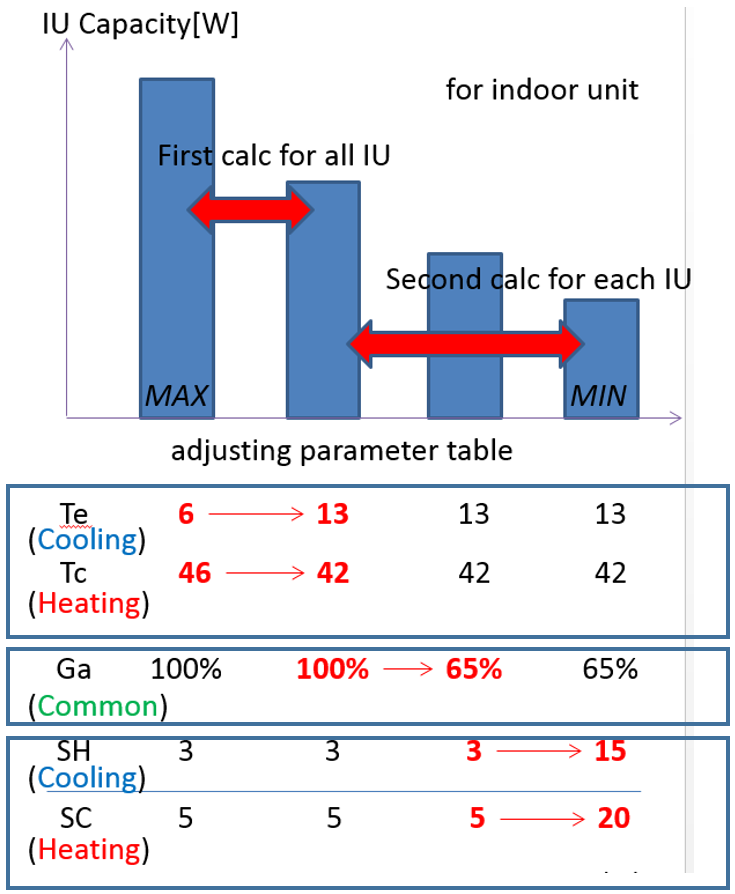
\includegraphics[width=0.45\textwidth, height=0.45\textheight, keepaspectratio=true]{media/VRF-FluidTCtrl-1a.png}
\caption{Multi-stage control strategy to adjust the system capacity during low load conditions \label{fig:multi-stage-control-strategy-to-adjust-the-system-capacity-during-low-load-conditions}}
\end{figure}

Note that a number of calculation steps are coupled together in the VRF-FluidTCtrl model, for instance, the piping loss calculation and the system performance calculation. More specifically, the piping loss changes the operating conditions of the system, which may lead to a different control strategy and thus in reverse affect the amount of piping loss. This makes it difficult to obtain an analytical solution for a number of operational parameters (e.g., enthalpy of refrigerant entering the indoor unit), and therefore numerical iterations are employed to address this problem (refer to Figure VRF-FluidTCtrl-3 for more details). Therefore, the VRF-FluidTCtrl model can have a longer execution time to perform the simulation than the VRF-SysCurve model.

The object connections for VRF-FluidTCtrl model is similar to those for VRF-SysCurve model. The difference lies in the object used to describe a specific components. For example, VRF-SysCurve model uses \emph{AirConditioner:VariableRefrigerantFlow} object to describe the VRF outdoor unit performance, while in VRF-FluidTCtrl model the \emph{AirConditioner:VariableRefrigerantFlow:FluidTemperatureControl} object is used.

\begin{figure}[hbtp] % figure VRF-FluidTCtrl-1b
\centering
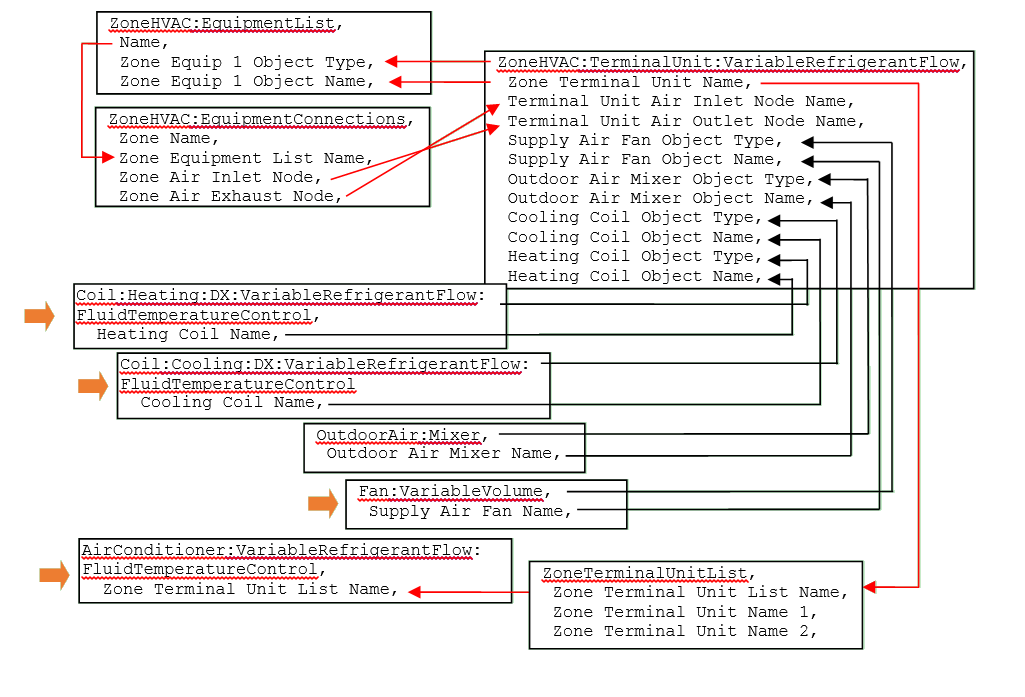
\includegraphics[width=0.9\textwidth, height=0.9\textheight, keepaspectratio=true]{media/VRF-FluidTCtrl-1b.png}
\caption{EnergyPlus object connections for VRF-FluidTCtrl model \label{fig:energyplus-object-connections-for-vrf-fluidtctrl-model}}
\end{figure}

\subsubsection{Model Description}\label{vrf-heat-pump-model-description}

Figures~\ref{fig:vrf-fluid-t-ctrl-2a}, \ref{fig:vrf-fluid-t-ctrl-2b}, \ref{fig:vrf-fluid-t-ctrl-3a}, and \ref{fig:vrf-fluid-t-ctrl-3b} illustrate the overall logic of the VRF-FluidTCtrl algorithms. Detailed calculation procedures and explanations of equations are described in the following sections.

\begin{figure}[hbtp] % figure VRF-FluidTCtrl-2a
\centering
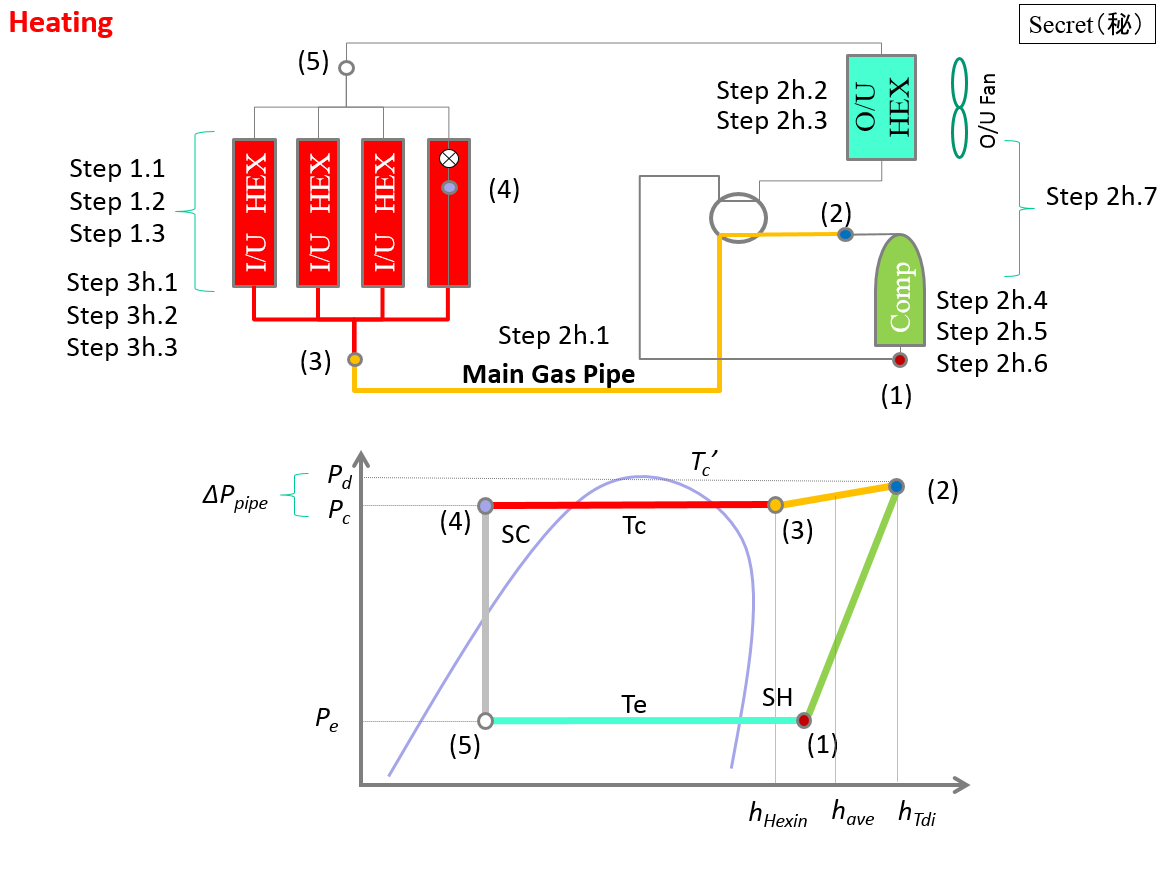
\includegraphics[width=0.9\textwidth, height=0.9\textheight, keepaspectratio=true]{media/VRF-FluidTCtrl-2a.png}
\caption{Schematic Pressure-Enthalpy Diagram for VRF Operation -- Heating Mode \label{fig:vrf-fluid-t-ctrl-2a}}
\end{figure}

\begin{figure}[hbtp] % figure VRF-FluidTCtrl-2b
\centering
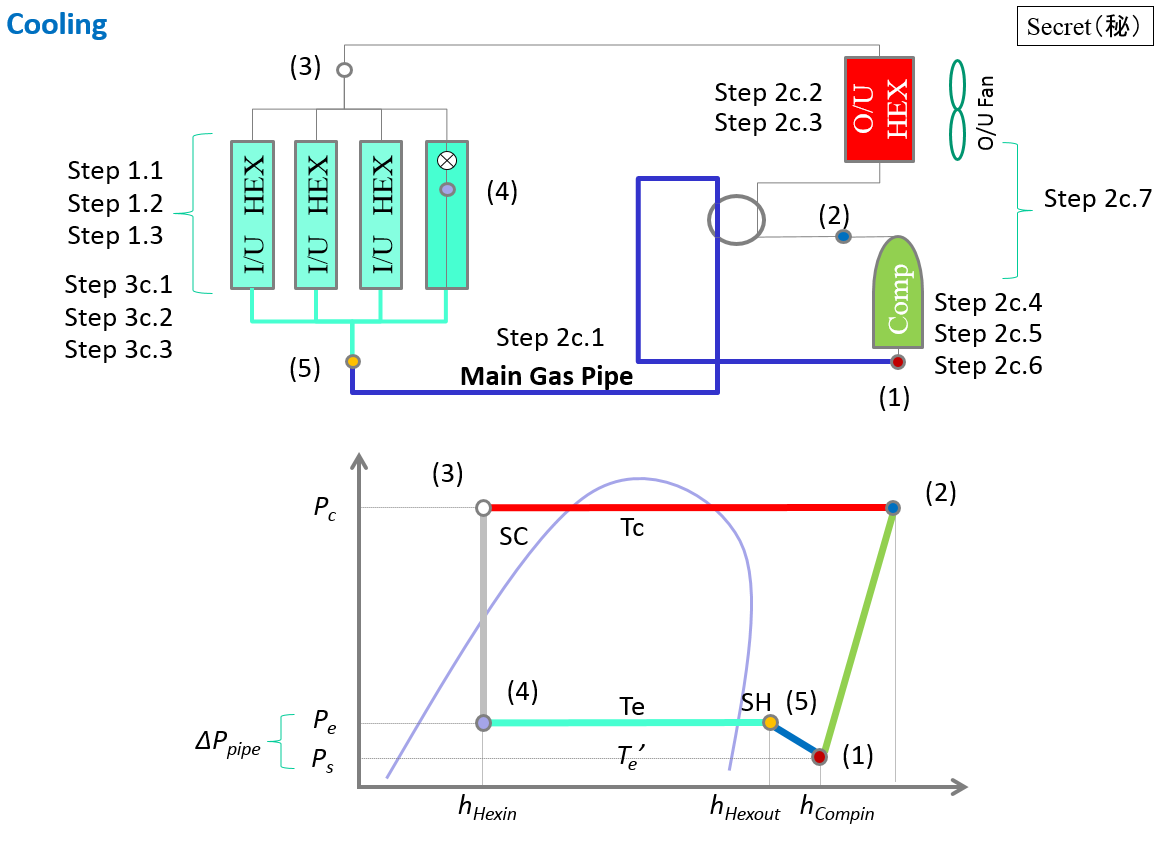
\includegraphics[width=0.9\textwidth, height=0.9\textheight, keepaspectratio=true]{media/VRF-FluidTCtrl-2b.png}
\caption{Schematic Pressure-Enthalpy Diagram for VRF Operation -- Cooling Mode \label{fig:vrf-fluid-t-ctrl-2b}}
\end{figure}

\begin{figure}[hbtp] % figure VRF-FluidTCtrl-3a
\centering
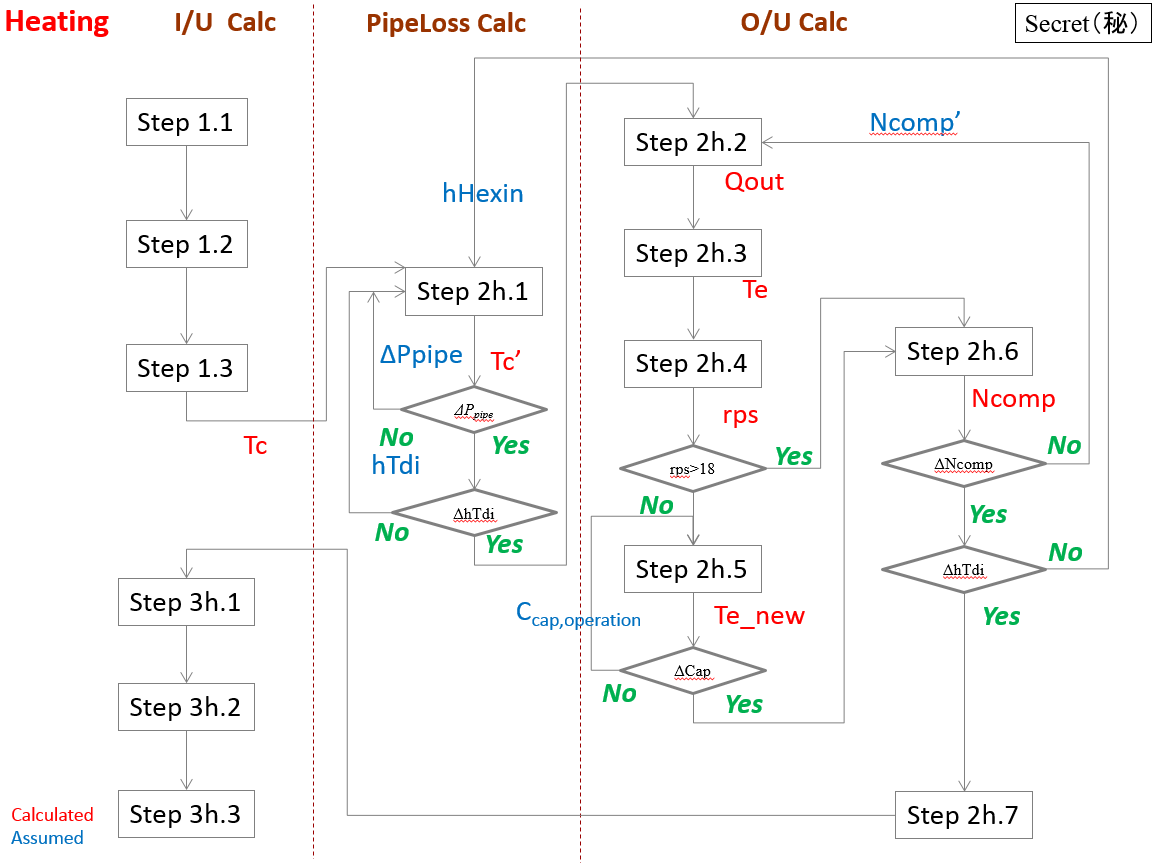
\includegraphics[width=0.9\textwidth, height=0.9\textheight, keepaspectratio=true]{media/VRF-FluidTCtrl-3a.png}
\caption{Flow Chart of the VRF-FluidTCtrl Model -- Heating Mode \label{fig:vrf-fluid-t-ctrl-3a}}
\end{figure}

\begin{figure}[hbtp] % figure VRF-FluidTCtrl-3b
\centering
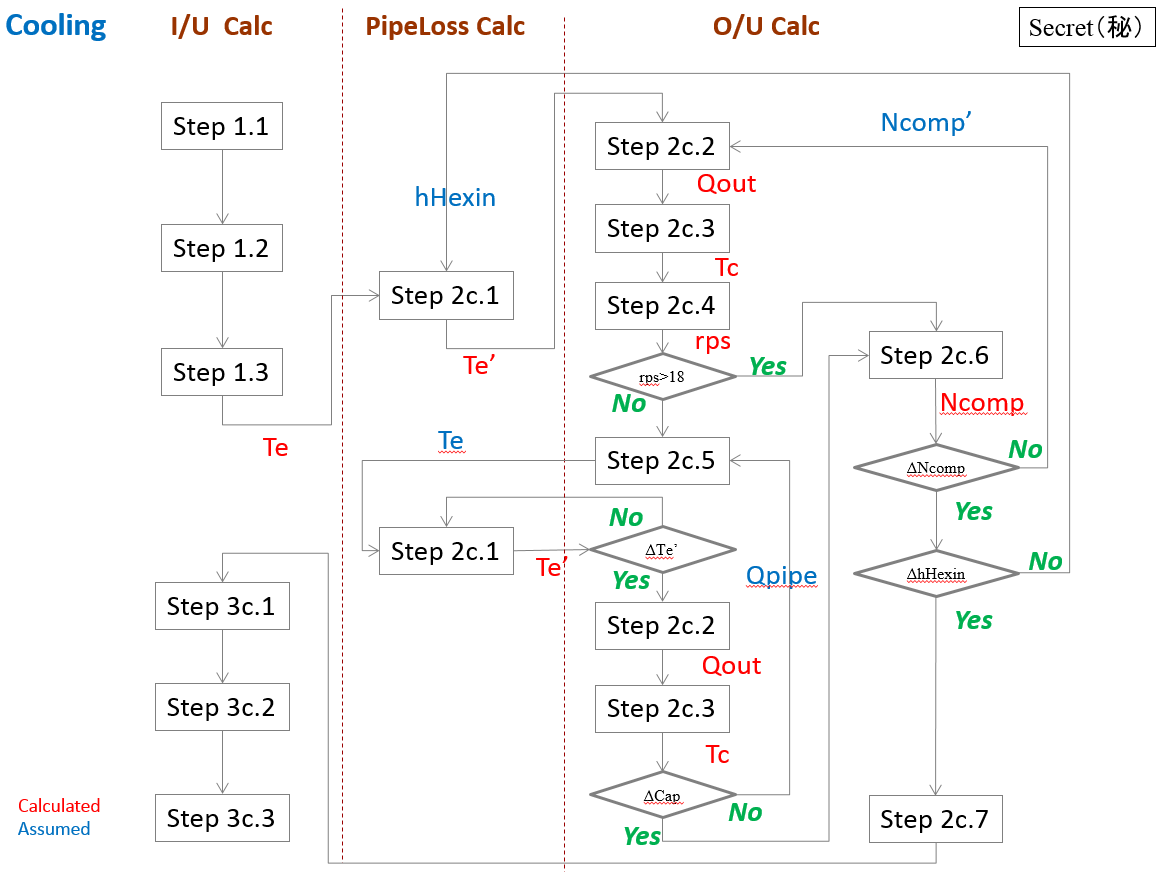
\includegraphics[width=0.9\textwidth, height=0.9\textheight, keepaspectratio=true]{media/VRF-FluidTCtrl-3b.png}
\caption{Flow Chart of the VRF-FluidTCtrl Model -- Cooling Mode \label{fig:vrf-fluid-t-ctrl-3b}}
\end{figure}

The VRF-FluidTCtrl algorithms are described in details below, including the models of both the indoor and outdoor unit(s) of the VRF system. Because of the different control algorithms used in the outdoor unit for cooling and heating modes, the heating and cooling modes are described separately.

\paragraph{Modeling of the indoor unit (I/U) -- Part I}\label{modeling-of-the-indoor-unit-iu-part-i}

\textbf{Step 1.1: Obtaining zonal load/condition information}

Obtain the following information for each zone from the zone modules within EnergyPlus:

\begin{itemize}
  \item
    zone sensible loads $Q_{in, sensible}$
  \item
    zone total loads $Q_{in, total}$
  \item
    indoor air temperature $T_{in}$
  \item
    indoor air humidity ratio $W_{in}$
\end{itemize}

The operation mode of the VRF system can therefore be determined from $Q_{in, sensible}$.

\textbf{Step 1.2: Calculate I/U required evaporator/condenser temperature}

Evaluate the required coil surface air temperature $T_{fs}$ and the required evaporator/condenser refrigerant temperature $T_{e,req}/{T_{c,req}}$ for each indoor unit.

Assuming the coil air flow rate is at the maximum ($G_{a,rate}$), the entering air temperature after the indoor coil fan can be calculated for each indoor unit:

\begin{equation}
  T_{coil,in}=T_{in}+Q_{fan}/(G_{a,rate}\times{c_p}\times\rho_{in})
\end{equation}

where:

$c_p$ is the air heat capacity (kJ/(kg$\cdot$K))

$G_{a,rate}$	 is the volumetric flow rate of the air through the indoor unit, at the rated conditions (m\(^3\)/s)

$Q_{fan}$ is the sensible heat released by fan (W)

$T_{coil,in}$ is the temperature of air entering the indoor coil (°C)

$\rho_{in}$ is the density of indoor air, $f_{\rho}(T_{in},W_{in})$ (kg/m\(^3\)).

The supply air temperature $T_{out}$ can be calculated by:

\begin{equation}
  T_{out} = T_{coil,in} - Q_{in, sensible} / (G_{a,rate}\times{c_p}\times\rho_{in})
\end{equation}

where $T_{out}$ is the temperature of the air leaving the indoor unit (supply air) (\(^{\circ}\)C).

The coil surface air temperature $T_{fs}$ can be calculated, given the bypass factor $BF$:

\begin{equation}
  T_{fs}= T_{coil,in} - (T_{coil,in}-T_{out}) / (1-BF)
\end{equation}

where:

$BF$ is the bypass factor (different values for cooling mode and heating mode)

$T_{fs}$ is the indoor unit coil surface air temperature (\(^{\circ}\)C).

In the cooling mode, the superheating degree $SH$ is given and thus the required evaporating temperature $Te_{req}$ for the associated indoor unit can be obtained:

\begin{equation}
  Te_{req}=T_{fs}-[A_c\cdot SH^2+B_c\cdot SH+C_c]
\end{equation}

Where

$A_c$, $B_c$, $C_c$ are coefficients

$SH$ is the superheating degrees for the indoor unit (\(^{\circ}\)C)

$SH_{ref}$ is the reference superheating degrees for the indoor unit (e.g., 3) (\(^{\circ}\)C)

$Te_{req}$ is the required evaporating temperature for a specific indoor unit (\(^{\circ}\)C).

In the heating mode, the subcooling degree $SC$ is given and thus the required condensing temperature $Tc_{req}$ for the associated indoor unit can be obtained:

\begin{equation}
  Tc_{req}=T_{fs}+[A_h\cdot SC^2+B_h\cdot SC+C_h]
\end{equation}

where:

$A_h$, $B_h$, $C_h$ are coefficients

$SC$ is the subcooling degrees for the indoor unit (\(^{\circ}\)C)

$SC_{ref}$ is the reference subcooling degrees for the indoor unit (e.g., 5) (\(^{\circ}\)C)

$Tc_{req}$ is the required condensing temperature for a specific indoor unit (\(^{\circ}\)C).

\textbf{Step 1.3: Calculate effective evaporating /condensing temperature}

There are two refrigerant temperature control strategies for the indoor unit: (1) \emph{ConstantTemp}, (2) \emph{VariableTemp}.

\begin{itemize}
  \item
    In the \emph{ConstantTemp} strategy, $T_e$ and $T_c$ are kept at constant values provided by the user.

 \item
   In the {VariableTemp} strategy, $T_e$ and $T_c$ are determined using the equations below:
\end{itemize}

In the cooling mode:

\begin{equation}
  Te = min \{ max [ min(Te_{req,i}), Te_{min}], Te_{max}\}
\end{equation}

where:

$Te_{req,i}$ is the required evaporating temperature for the ith indoor unit (\(^{\circ}\)C)

$Te_{min}$ is the minimum evaporating temperature for the indoor unit (e.g. 3) (\(^{\circ}\)C)

$Te_{max}$ is the maximum evaporating temperature for the indoor unit (e.g. 13) (\(^{\circ}\)C).

In the heating mode:

\begin{equation}
  Tc = min \{ max[min(Tc_{req,i}),Tc_{min}],Tc_{max} \}
\end{equation}

where:

$Tc_{req,i}$ is the required condensing temperature for the ith indoor unit (\(^{\circ}\)C)

$Tc_{min}$ is the minimum condensing temperature for the indoor unit (e.g. 42) (\(^{\circ}\)C)

$Tc_{max}$ is the maximum condensing temperature for the indoor unit (e.g. 46) (\(^{\circ}\)C).

\paragraph{Modeling of the outdoor unit (O/U) - Cooling Mode}\label{modeling-of-the-outdoor-unit-ou-cooling-mode}

\textbf{Step 2c.1: Piping loss calculation in the cooling mode}

Piping loss occurs when the refrigerant flows through the main pipe connecting the indoor and outdoor units. It includes both the refrigerant pressure drop and heat loss. It affects the VRF system operation in several ways. First, the heat loss creates an extra load to the system and leads to higher energy consumptions. Second, the pressure drop and heat loss changes the operational conditions of the compressor (i.e., compressor suction pressure and compressor suction temperature) and thus affects its operational performance. Therefore, the piping loss calculation is critical for the analysis of the whole system.

Note that the change of compressor operational conditions may lead to different control strategies of the system, which in reverse affects the amount of piping loss. So the piping loss analysis and system performance analysis are coupled together. Numerical iterations are designed to address the coupling effect, as described below.

Calculate the refrigerant flow rate for each indoor unit using assumed $h_{Hexin}$:

\begin{equation}
  G_i=Q_i/(h_{Hexout,i}-h_{Hexin})
\end{equation}

where:

$G_i$ is the refrigerant flow rate for the i\(^{th}\) indoor unit (kg/s)

$Q_i$ is the total cooling load of the i\(^{th}\) zone (W)

$h_{Hexin}$ is the enthalpy of the refrigerant entering the indoor unit (kJ/kg)

$h_{Hexout,i}$ is the enthalpy of the refrigerant leaving a specific indoor unit (kJ/kg)

$h_{Hexout,i}$ is a function of $P_e$, $T_e$, and $SH_i$. It can be calculated using refrigerant thermodynamic property equations $f_{g\_h}(P_e,T_e+SH_i)$.

The enthalpy of the refrigerant in the main loop $h_{Hexout}$ can be obtained by calculating the weighted average of the enthalpy of the refrigerant in each indoor unit:

\begin{equation}
  h_{Hexout}=\sum(h_{Hexout,i}\times{G_i}/{G_{tot}})
\end{equation}

\begin{equation}
  G_{tot}=\sum{G_i}
\end{equation}

where:

$G_{tot}$ is the refrigerant flow rate in the main loop (kg/s)

$h_{Hexout}$ is the enthalpy of the main loop refrigerant leaving indoor units (kJ/kg).

The viscosity of the refrigerant within the pipe can be calculated via:

\begin{equation}
  k_{v,1}=P_e/4926000
\end{equation}

\begin{equation}
  k_{v,2}=h_{Hexout}/383.55
\end{equation}

\begin{equation}
  k_{v,3}=(T_{Hexout}+273.15)/344.39
\end{equation}

\begin{equation}
\begin{array}{rl}
\mu =& 10^6\times(4.302\times{k_{v,1}}+0.81622\times{k_{v,1}}^2-120.98\times{k_{v,2}}+139.17\times{k_{v,2}}^2 \\
 & +118.76\times{k_{v,3}}+81.04\times{k_{v,3}}^2+5.7858\times{k_{v,1}}\times{k_{v,2}} \\
 & -8.3817\times{k_{v,1}}\times{k_{v,3}}-218.48\times{k_{v,2}}\times{k_{v,3}}+21.58)
\end{array}
\end{equation}

where:

$\mu$ is the viscosity of the refrigerant within the pipe (Pa-s)

$k_{v,i}$ is the coefficients to calculate the refrigerant viscosity

$T_{Hexout}$ is the temperature of main loop refrigerant leaving indoor units, $f_{g\_t}(P_e,h_{Hexout})$ (\(^{\circ}\)C)

$f_{g\_t}$ are functions calculating the temperature of superheating refrigerant.

Given $h_{Hexout}$ and $P_e=f_{s\_p}(T_e)$, the following dimensionless quantities describing the refrigerant flow state can be obtained:

\begin{equation}
  Re=G_{tot}/3600/(0.25\times\pi\times{D^2})\times{D}/\mu
\end{equation}

\begin{equation}
  Pr=\mu\times{f_{g\_Cp}(P_e,h_{Hexout})}\times{0.001}/f_{g\_\lambda}(P_e,h_{Hexout})
\end{equation}

\begin{equation}
  Nu=0.023\times{Re^{0.8}\times{Pr^{0.3}}}
\end{equation}

\begin{equation}
  St=Nu/Re/Pr
\end{equation}

where:

$P_e$ is the evaporating pressure (Pa)

$Re$ is the Reynolds number

$Pr$ is the Prandtl number

$Nu$ is the Nusselt number

$St$ is the Stanton number

$\mu$ is the viscosity of the refrigerant within the pipe (Pa-s)

$f_{s\_p}$ are functions calculating the pressure of saturated refrigerant

$f_{g\_Cp}$ are functions calculating the specific heat of superheating refrigerant

$f_{g\_\lambda}$ are functions calculating the conductivity of superheating refrigerant.

Then the piping pressure loss $\Delta{P_{pipe}}$ can be obtained using the above dimensionless quantities:

\begin{equation}
  \Delta{P_{pipe}}=8\times{St}\times{Pr^{2/3}}\times{L/D}\times{f_{g\_\rho}(P_e,h_{Hexout})}\times{V^2}/2+H\times{f_{g\_\rho}(P_e,h_{Hexout})}\times9.80665
\end{equation}

\begin{equation}
  P_s=P_e-\Delta{P_{pipe}}
\end{equation}

where:

$f_{g\_\rho}$ are functions calculating the density of superheating refrigerant

$D$ is the main pipe diameter (m)

$H$ is the height difference between the outdoor unit node and indoor unit node of the main pipe (m)

$L$ is the main pipe length (outdoor unit to the first branch joint) (m)

$P_s$ is the compressor suction pressure (Pa)

$\Delta{P_{pipe}}$ is the pressure drop in the pipe (Pa)

$V$ is the refrigerant flow velocity (m/s).

The suction saturated temperature $T'_e$ (i.e., saturated vapor temperature corresponding to the compressor suction pressure) can be obtained via refrigerant thermodynamic property equations:

\begin{equation}
  T'_e=f_{s\_t}(P_e-\Delta{P_{pipe}})
\end{equation}

where:

$f_{s\_t}$ are functions calculating the temperature of saturated refrigerant

$T'_e$ is the suction saturated temperature at the compressor inlet (\(^{\circ}\)C).

The heat loss through the pipe can be obtained via:

\begin{equation}
k_1=Nu\times{f_{g\_\lambda}(P_e,h_{Hexout})}
\end{equation}

\begin{equation}k_2=2\times{\lambda_i}/Ln(1+2\times{W_i}/D)\end{equation}

\begin{equation}k_3=h\times(D+2\times{W_i})\end{equation}

\begin{equation}Q_{pipe}=(\pi\times{L})\times(T_a-T_{Hexout})/(1/k_1+1/k_2+1/k_3)\end{equation}

where:

$f_{g\_\lambda}$ are functions calculating the conductivity of superheating refrigerant

$Q_{pipe}$ is the heat loss through the pipe (W)

$T_a$ is the average of outdoor air temperature and indoor temperature (\(^{\circ}\)C)

$T_{Hexout}$ is the temperature of main pipe refrigerant leaving indoor units (\(^{\circ}\)C)

$w_i$ is the pipe insulation thickness (m)

$k_i$ are coefficients for the piping loss calculation.

Note that $Q_{pipe}$ is calculated using an assumed $h_{Hexin}$. Its value affects the compressor operation calculations as shown in Steps 2c.2 - 2c.6 and may change the value of condensing temperature $T_c$. This leads to an updated $h_{Hexin}=f(P_c,T_c-SC)$. If the difference between the calculated $h_{Hexin}$ and the assumed $h_{Hexin}$ is higher than the assigned tolerance (5\%), a new round of iteration is performed using the calculated $h_{Hexin}$.

\textbf{Step 2c.2: Initialize O/U operation conditions}

The compressor operation is coupled with a number operational parameters, which makes it difficult to obtain an analytical solution. In the algorithm, an iterative approach is designed to obtain the energy consumption of the compressor (Step 2c.2 – 2c.6).

For the first iteration,

\begin{itemize}
  \item
    Initialize outdoor unit $SC$ with the reference value (from IDF input, e.g., 5\(^{\circ}\)C)
  \item
    Initialize the compressor power $N_{comp}$ with the value calculated from the reference $COP$ (e.g., 3.5):
\end{itemize}

\begin{equation}N'_{comp}=\frac{\sum_iQ_{in,total,i}}{COP}\end{equation}

where:

$N_{comp}$ is the compressor power (W)

$N'_{comp}$ is the assumed compressor power for the first iteration (W)

$Q_{in,total,i}$ is the total cooling load for zone $i$ (W).

For the following iterations,

\begin{itemize}
\item Initialize $SC$ with the calculated value in the previous iteration
\item Initialize the compressor power $N_{comp}$ with the calculated value in the previous iteration
\end{itemize}

The heat rate released from the outdoor unit can be calculated by:

\begin{equation}Q_{out}=\sum_iQ_{in,total,i}+N_{comp}+Q_{pipe}\end{equation}

where:

$Q_{out}$ is the heat rate released from the outdoor unit (W)

$Q_{pipe}$ is the heat loss through the pipe (W).

\textbf{Step 2c.3: Calculate O/U effective condensing temperature}

 (1) Calculate the required coil surface air temperature ${T_{fs}}'$ for the outdoor unit.

The temperature of the air leaving the outdoor unit ${T_{out}}'$ can be calculated by:

\begin{equation}{T_{out}}'={T_{in}}'+Q_{out}/({G_{a,rate}}'\times{c_p}\times{{\rho_{in}}'})\end{equation}

where:

${G_{a,rate}}'$ is the volumetric flow rate of the air through the outdoor unit, at the rating conditions (m\(^3\)/s)

${T_{out}}'$ is the temperature of the air leaving the outdoor unit (\(^{\circ}\)C)

${T_{in}}'$ is the temperature of the air entering the outdoor unit, i.e., outdoor air (\(^{\circ}\)C)

${\rho_{in}}'$ is the air density at outdoor conditions, $f_{\rho}({T_{in}}',{W_{in}}')$ (kg/m\(^3\)).

The condenser surface temperature ${T_{fs}}'$ can be calculated by:

\begin{equation}{T_{fs}}'={T_{in}}'+({T_{out}}'-{T_{in}}')/(1-{BF_c}')\end{equation}

where ${BF_c}'$ is the bypass factor for the outdoor unit.

(2) Calculate required condensing temperature for the outdoor unit $Tc_{req}$ and then the effective condensing temperature $Tc$ (between 42-46\(^{\circ}\)C)

\begin{equation}
Tc_{req}={T_{fs}}'+[A_h\cdot SC^2+B_h\cdot SC+C_h]
\end{equation}

\begin{equation}
Tc=Tc_{req}
\end{equation}

where:

$A_h$, $B_h$, $C_h$ are coefficients

$SC$ is the subcooling degrees for the outdoor unit (\(^{\circ}\)C)

$SC_{ref}$ is the reference subcooling degrees for the outdoor unit (\(^{\circ}\)C)

$Tc_{req}$ is the required condensing temperature for the outdoor unit (\(^{\circ}\)C)

$Tc$ is the effective condensing temperature (\(^{\circ}\)C).

\textbf{Step 2c.4: Calculate required Loading Index}

Loading Index is used to describe the operational mode of the compressor system. The first index represents minimal capacity operation, while the last index represents full capacity operation.

The required Loading Index can be calculated by the following procedures.

\begin{enumerate}
\def\labelenumi{\alph{enumi}.}
\tightlist
\item Calculate the evaporative capacity at a variety of Loading Index:
\end{enumerate}

\begin{equation}
M_{cap}=(r_1+r_2T_c+r_3{T_e}'+r_4T_c^2+r_5T_c{T_e}'+r_6{T_e}'^2)
\end{equation}

\begin{equation}
Q_{rps}=C_{cap,system} \times M_{cap} \times Q_{ref}
\end{equation}

where:

$C_{cap,system}$ is the evaporative capacity correction factor, describing the possible system configuration difference between test bed and real system (a constant value obtained from manufacturer data)

$r_1$, \ldots, $r_6$ are the empirical coefficients corresponding to $rps$

$rps$ is the compressor speed (r/s)

${T_e}'$ is the suction saturated temperature at the compressor inlet (\(^{\circ}\)C)

$T_c$ is the effective condensing temperature (\(^{\circ}\)C)

$M_{cap}$ is the multiplier for the evaporative capacity calculation (--)

$Q_{rps}$ is the evaporative capacity corresponding to $rps$ (W)

$Q_{ref}$ is the rated evaporative capacity (W).

An example of resulting capacity for different $rps$ (at $T_c$=36\(^{\circ}\)C and ${T_e}'$=9\(^{\circ}\)C) is presented in Table~\ref{table:evaporative-capacity-at-different-loading-index}.

\begin{longtable}[c]{>{\raggedright}p{1.5in}>{\raggedright}p{1.5in}>{\raggedright}p{1.5in}>{\raggedright}p{1.5in}}
\caption{Evaporative capacity at different Loading Index \label{table:evaporative-capacity-at-different-loading-index}} \tabularnewline
\toprule
Loading Index ($rps$) & Evaporative Capacity (kW), $T_c$=36\(^{\circ}\)C, ${T_e}'$=9\(^{\circ}\)C & Loading Index ($rps$) & Evaporative Capacity (kW), $T_c$=36\(^{\circ}\)C, ${T_e}'$=9\(^{\circ}\)C \tabularnewline
\midrule
\endfirsthead

\caption[]{Evaporative capacity at different Loading Index} \tabularnewline
\toprule
Loading Index ($rps$) & Evaporative Capacity (kW), $T_c$=36\(^{\circ}\)C, ${T_e}'$=9\(^{\circ}\)C & Loading Index ($rps$) & Evaporative Capacity (kW), $T_c$=36\(^{\circ}\)C, ${T_e}'$=9\(^{\circ}\)C \tabularnewline
\midrule
\endhead

1 (18)  & 3.951  & 2 (25) & 5.400  \tabularnewline
3 (30)  & 6.435  & 4 (36) & 8.516  \tabularnewline
5 (45)  & 10.756 & 6 (60) & 14.445 \tabularnewline
7 (75)  & 18.412 & 8 (90) & 22.045 \tabularnewline
9 (108) & 26.162 &        &        \tabularnewline
\bottomrule
\end{longtable}

\begin{enumerate}
\def\labelenumi{\alph{enumi}.}
\setcounter{enumi}{1}
\tightlist
\item
  Find the \(rps\) range that covers the required evaporative capacity \(Q_{rps,modify}\) .
\end{enumerate}

\begin{equation}
Q_{rps,modify} = C_{cap,operation}\times(\sum{Q_{in,total}}+Q_{pipe})
\end{equation}

\begin{equation}
C_{cap,operation} = C_{cap,density}\times{C_{cap,enthalpy}}
\end{equation}

\begin{equation}
C_{cap,density} = \rho_{test}/\rho_{real}
\end{equation}

\begin{equation}
C_{cap,enthalpy} = \frac{h_{Evapout,test}-h_{Evapin,test}}{h_{Compin,real}-h_{Evapin,real}}
\end{equation}

\begin{equation}
h_{Compin,real} = h_{Hexout,real}+Q_{pipe}/G_{tot}
\end{equation}

where:

\(C_{cap,operation}\) is the evaporative capacity correction factor, describing the operational difference between test cases and real cases (i.e., \(SH\) and \(SC\) )

\(C_{cap,density}\) is the evaporative capacity correction factor, describing the variations of refrigerant density at test conditions and real operational conditions

\(C_{cap,enthalpy}\) is the evaporative capacity correction factor, describing the variations of refrigerant enthalpy at test conditions and real operational conditions

\(G_{tot}\) is the refrigerant flow rate in the main loop (kg/s)

\(h_{Evapin,real}\) is the enthalpy of refrigerant entering the evaporators (IU) at real conditions (kJ/kg)

\(h_{Evapout,real}\) is the average enthalpy of refrigerant leaving the evaporators (IU) at real conditions (kJ/kg)

\(h_{Evapin,test}\) is the enthalpy of refrigerant entering the evaporator at test conditions (i.e., \(SC\) at test conditions (e.g., 5\(^{\circ}\)C) and Tc) (kJ/kg)

\(h_{Evapout,test}\) is the enthalpy of refrigerant leaving the evaporator at test conditions (i.e., \(SH\) at test conditions (e.g., 8\(^{\circ}\)C) and Te) (kJ/kg)

\(h_{Compin}\) is the enthalpy of refrigerant entering the compressor (kJ/kg)

\(Q_{pipe}\) is the heat loss through the pipe (W).

For example, if the required capacity is 8 kW, the \(rps\) range is 30 to 36.

\begin{enumerate}
\def\labelenumi{\alph{enumi}.}
\setcounter{enumi}{2}
\item
  Calculate the \(rps\) that meets the required capacity by interpolation. In the above example, the resulting \(rps\) is 34.5 \(rps\).
\item
  If the calculated \(rps\) is lower than the minimum \(rps\) (e.g.~18~\(rps\) ), go to Step 2c.5, otherwise skip Step 2c.5 and directly go to Step 2c.6.
\end{enumerate}

\textbf{Step 2c.5: Modify evaporating temperature to further reduce outdoor unit capacity}

If the calculated \(rps\) is lower than the minimum \(rps\) (e.g.~18~\(rps\) ), it means that the zone cooling load is even lower than the system evaporative capacity corresponding to the minimum compressor speed. In this situation, the evaporating temperature \(T_e\) as well as the superheating degree \(SH\) is modified to further reduce the outdoor unit capacity. More specifically:

\begin{enumerate}
\def\labelenumi{\alph{enumi}.}
\item
  Set \(rps\) at its minimum value (e.g., 18~\(rps\)).
\item
  Update \({T_e}'\) to meet the required evaporative capacity, using equations described in Step 2c.4a.
\item
  Update \(T_e\) to meet the updated \({T_e}'\) . Note that due to the \(T_e\) updates, the refrigerant state and flow rate are changed and thus the piping loss analysis should also be repeated (Step 2c.1). So is the calculation of \(C_{cap,operation}\) (Step 2c.2 - 2c.3).
\item
  \(SH\) can be updated based on the updated \(T_e\), using the equations shown in Step 1.2.
\end{enumerate}

\textbf{Step 2c.6: Calculate the compressor power}

\begin{enumerate}
\def\labelenumi{(\arabic{enumi})}
\tightlist
\item
  Calculate the compressor power by the following procedures.
\end{enumerate}

\begin{enumerate}
\def\labelenumi{\alph{enumi}.}
\tightlist
\item
  Calculate the compressor power at a variety of loading index using the following equation. The resulting table from the same example used above is shown below in Table~\ref{table:outdoor-unit-compressor-power-at-different-loading-index-20160504}.
\end{enumerate}

\begin{equation}
  M_{comp} = c_1+c_2T_c+c_3{T_e}'+c_4T_c^2+c_5T_c{T_e}'+c_6{T_e}'^2
\end{equation}

\begin{equation}
  N_{comp,rps} = M_{comp} \times N_{comp,ref}
\end{equation}

where:

\(c_1\),~\ldots{},~\(c_6\) are the empirical coefficients corresponding to \(rps\)

\({T_e}'\) is the suction saturated temperature at the compressor inlet (\(^{\circ}\)C)

\(T_c\) is the effective condensing temperature (\(^{\circ}\)C)

\(M_{comp}\) is the multiplier for the compressor power calculation (--)

\(N_{comp,ref}\) is the rated compressor power (W)

\(N_{comp,rps}\) is the compressor power corresponding to \(rps\) (W).

\begin{longtable}[c]{ll}
\caption{Outdoor unit compressor power at different Loading Index \label{table:outdoor-unit-compressor-power-at-different-loading-index-20160504}} \tabularnewline
\toprule
Loading Index (\(rps\)) & Evaporative Capacity (kW), \(T_c\)=36\(^{\circ}\)C, \({T_e}'\)=9\(^{\circ}\)C \tabularnewline
\midrule
\endfirsthead

\caption[]{Outdoor unit compressor power at different Loading Index} \tabularnewline
\toprule
Loading Index ($rps$) & Evaporative Capacity (kW), $T_c$=36\(^{\circ}\)C, ${T_e}'$=9\(^{\circ}\)C \tabularnewline
\midrule
\endhead

1 (18)  & 3.951  \tabularnewline
2 (25)  & 5.400  \tabularnewline
3 (30)  & 6.435  \tabularnewline
4 (36)  & 8.516  \tabularnewline
5 (45)  & 10.756 \tabularnewline
6 (60)  & 14.445 \tabularnewline
7 (75)  & 18.412 \tabularnewline
8 (90)  & 22.045 \tabularnewline
9 (108) & 26.162 \tabularnewline
\bottomrule
\end{longtable}

\begin{enumerate}
\def\labelenumi{\alph{enumi}.}
\setcounter{enumi}{1}
\tightlist
\item
  According to the \(rps\) range determined, calculate the compressor power \(N_{comp}\) by interpolation. In the above example, the compressor power is 1.155 kW.
\end{enumerate}

\begin{enumerate}
\def\labelenumi{(\arabic{enumi})}
\setcounter{enumi}{1}
\tightlist
\item
  Compare the calculated \(N_{comp}\) above with the initialized \({N_{comp}}'\) in Step 2c.2:
\end{enumerate}

\begin{itemize}
\item
  If \({N_{comp}}'-N_{comp}>\delta\) then go to Step 2c.2 for a new round of iteration.
\item
  Else, end the iteration and go to Step 2c.7.
\end{itemize}

\textbf{Step 2c.7: Total power consumption of the outdoor unit}\label{step-2c.7-total-power-consumption-of-the-outdoor-unit}

Calculate the total electric power consumption by the outdoor unit:

\begin{equation}
N_{out} = N_{fan}+N_{comp}/e_{inv}
\end{equation}

where:

\(e_{inv}\) is the efficiency of the inverter of compressor

\(N_{fan}\) is the electric power consumption by the outdoor fan (W)

\(N_{out}\) is the total electric power consumption by the outdoor unit (W).

\subsubsection{\emph{Modeling of the outdoor unit (O/U) - Heating Mode}}\label{modeling-of-the-outdoor-unit-ou---heating-mode}

\textbf{Step 2h.1: Piping loss calculation in the heating mode}

Similarly to that in the cooling mode, the piping loss analysis in the heating mode needs to address the coupling effect between the piping loss and system operations. However, due to the control strategy difference between the two modes, the piping loss algorithm in the heating mode requires different calculation steps and more numerical iterations, as shown below.

Calculate the refrigerant flow rate for each indoor unit using assumed \(h_{Hexin}\):

\begin{equation}
G_i = Q_i/(h_{Hexin}-h_{Hexout,i})
\end{equation}

where:

\(G_i\) is the refrigerant flow rate for the i\(^{th}\) indoor unit (kg/s)

\(Q_i\) is the total heating load of the i\(^{th}\) zone (W)

\(h_{Hexin}\) is the enthalpy of the refrigerant entering the indoor unit (kJ/kg)

\(h_{Hexout,i}\) is the enthalpy of the refrigerant leaving a specific indoor unit (kJ/kg)

\(h_{Hexout,i}\) is a function of \(P_c\), \(T_c\), and \(SC_i\). It can be calculated using refrigerant thermodynamic property equations \(f_{g_h}(P_c,T_c-SC_i)\).

The refrigerant flow rate in the main loop can be obtained by summing up the flow rate in each indoor unit:

\begin{equation}
G_{tot} = \sum{G_i}
\end{equation}

where \(G_{tot}\) refrigerant flow rate in the main loop (kg/s).

Calculate the average refrigerant pressure and enthalpy within the pipes, using assumed piping pressure loss \(\Delta{P_{pipe}}\) and \(h_{Tdi}\) :

\begin{equation}
P_{ave} = P_c+\Delta{P_{pipe}}/2
\end{equation}

\begin{equation}
h_{ave} = (h_{Hexin}+h_{Tdi})/2
\end{equation}

where:

\(h_{ave}\) is the average refrigerant enthalpy within the main pipe (kJ/kg)

\(h_{Hexin}\) is the enthalpy of the refrigerant entering the indoor unit (kJ/kg)

\(h_{Tdi}\) is the enthalpy of the refrigerant leaving the compressor (kJ/kg)

\(P_{ave}\) is the average refrigerant pressure within the main pipe (Pa)

\(P_c\) is the condensing pressure (Pa)

\(\Delta{P_{pipe}}\) is the pressure drop in the main pipe (Pa).

The viscosity of the refrigerant within the pipe can be calculated given \(P_{ave}\) and \(h_{ave}\), using the following equations:

\begin{equation}
k_{v,1} = P_{ave}/4926000
\end{equation}

\begin{equation}
k_{v,2} = h_{ave}/383.55
\end{equation}

\begin{equation}
k_{v,3} = (T_{ave}+273.15)/344.39
\end{equation}

\begin{equation}
\begin{array}{rl}
\mu =& 10^6\times(4.302\times{k_{v,1}}+0.81622\times{k_{v,1}}^2-120.98\times{k_{v,2}}+139.17\times{k_{v,2}}^2 \\
 & +118.76\times{k_{v,3}}+81.04\times{k_{v,3}}^2+5.7858\times{k_{v,1}}\times{k_{v,2}} \\
 & -8.3817\times{k_{v,1}}\times{k_{v,3}}-218.48\times{k_{v,2}}\times{k_{v,3}}+21.58)
\end{array}
\end{equation}

where:

\(\mu\) is the viscosity of the refrigerant within the pipe (Pa-s)

\(k_{v,i}\) are coefficients to calculate the refrigerant viscosity

\(h_{ave}\) is the average refrigerant enthalpy within the pipes (kJ/kg)

\(P_{ave}\) is the average refrigerant pressure within the pipes (Pa)

\(T_{ave}\) is the average temperature of refrigerant leaving indoor units, which corresponds to \(P_{ave}\) and \(h_{ave}\) (\(^{\circ}\)C)

Given \(P_{ave}\) and \(h_{ave}\), the following dimensionless quantities describing the refrigerant flow state can be obtained:

\begin{equation}
Re = G_{tot}/3600/(0.25\times\pi\times{D^2})\times{D}/\mu
\end{equation}

\begin{equation}
Pr = \mu\times{f_{g_{C_p}}(P_{ave},h_{ave})}\times{0.001}/f_{g_\lambda}(P_{ave},h_{ave})
\end{equation}

\begin{equation}
Nu = 0.023\times{Re^{0.8}\times{Pr^{0.4}}}
\end{equation}

\begin{equation}
St = Nu/Re/Pr
\end{equation}

where:

\(Re\) is the Reynolds number

\(Pr\) is the Prandtl number

\(Nu\) is the Nusselt number

\(St\) is the Stanton number

\(\mu\) is the viscosity of the refrigerant within the pipe (Pa-s)

\(f_{g_{C_p}}\) are functions calculating the specific heat of superheating refrigerant

\(f_{g_\lambda}\) are functions calculating the conductivity of superheating refrigerant.

Then, the piping pressure loss \(\Delta{P_{pipe}}\) can be obtained using the above dimensionless quantities:

\begin{equation}
\Delta{P_{pipe}} = 8\times{St}\times{Pr^{2/3}}\times{L/D}\times{f_{g_\rho}(P_{ave},h_{ave})}\times{V^2}/2-H\times{f_{g_\rho}(P_{ave},h_{ave})}\times9.80665
\end{equation}

where:

\(f_{g_\rho}\) are functions calculating the density of superheating refrigerant

\(D\) is the main pipe diameter (m)

\(H\) is the height difference between the outdoor unit node and indoor unit node of the main pipe (m)

\(L\) is the main pipe length (outdoor unit to the first branch joint) (m)

\(St\) is the Stanton number

\(Re\) is the Reynolds number

\(Pr\) is the Prandtl number

\(\Delta{P_{pipe}}\) is the pressure drop in the pipe (Pa)

\(V\) is the refrigerant flow velocity (m/s).

Compare the calculated \(\Delta{P_{pipe}}\) and the one assumed above. If the difference is higher than the assigned tolerance (5\%), a new round of iteration is performed using the calculated \(\Delta{P_{pipe}}\).

The compressor discharge saturated temperature \(T'_c\) (i.e., saturated vapor temperature corresponding to compressor discharge pressure) can be obtained via:

\begin{equation}
T'_c = f_{s_t}(P_c+\Delta{P_{pipe}})
\end{equation}

where:

\(f_{s_t}\) are functions calculating the temperature of saturated refrigerant

\(T'_c\) is the discharge saturated temperature at the compressor outlet (\(^{\circ}\)C)

\(P_c\) is the condensing pressure (Pa)

\(\Delta{P_{pipe}}\) is the pressure drop in the pipe (Pa).

The heat loss through the pipe can be obtained via:

\begin{equation}
k_1 = Nu\times{f_{g_\lambda}(P_{ave},h_{ave})}
\end{equation}

\begin{equation}
k_2 = 2\times{\lambda_i}/Ln(1+2\times{W_i}/D)
\end{equation}

\begin{equation}
k_3 = h\times(D+2\times{W_i})
\end{equation}

\begin{equation}
Q_{pipe} = (\pi\times{L})\times(T_a-T_{Hexin})/(1/k_1+1/k_2+1/k_3)
\end{equation}

where:

\(f_{g_\lambda}\) are functions calculating the conductivity of superheating refrigerant

\(Q_{pipe}\) is the heat loss through the pipe (W)

\(T_a\) is the average of outdoor air temperature and indoor temperature (\(^{\circ}\)C)

\(T_{Hexin}\) is the average of entering indoor units (\(^{\circ}\)C)

\(w_i\) is the pipe insulation thickness (m)

\(k_i\) is the coefficients for the piping loss calculation.

The enthalpy of the refrigerant entering the indoor unit can be updated using the calculated \(Q_{pipe}\):

\begin{equation}
h_{Tdi} = h_{Hexin}+Q_{pipe}/G_{tot}
\end{equation}

where:

\(h_{Hexin}\) is the enthalpy of the refrigerant entering the indoor unit (kJ/kg)

\(h_{Tdi}\) is the enthalpy of the refrigerant leaving the compressor (kJ/kg)

\(G_{tot}\) is the refrigerant flow rate in the main loop (kg/s).

Compare the calculated \(h_{Tdi}\) and the one assumed above. If the difference is higher than the assigned tolerance (5\%), a new round of iteration is performed using the calculated \(h_{Tdi}\).

Note that \(Q_{pipe}\) is calculated using an assumed \(h_{Hexin}\) at the beginning of the piping loss algorithm. Its value affects the compressor operation calculations as shown in Step 2h.2\textasciitilde{}2h.6 and may change the value of evaporating temperature \(T_e\). This leads to an updated \(h_{Hexin} = f(P_e,T_e+SH,N_{comp},G_{tot})\). If the difference between the calculated result and the assumed value is higher than the assigned tolerance (5\%), a new round of iteration is performed using the calculated \(h_{Hexin}\).

\textbf{Step 2h.2: Initialize O/U operation conditions}

Similar to that in cooling mode, an iteration approach is designed to determine the energy consumption of the compressor (Step 2h.2 to Step 2h.6).

For the first iteration,

\begin{itemize}
\item
  Initialize outdoor unit \(SH\) with the reference value (from IDF input, e.g., 1.5\(^{\circ}\)C)
\item
  Iinitialize the compressor power \(N_{comp}\) with the value calculated from the reference \(COP\) (e.g., 3.5):
\end{itemize}

\begin{equation}
N'_{comp} = \frac{\sum_iQ_{in,total,i}}{COP}
\end{equation}

where:

\(N_{comp}\) is the compressor power (W)

\(N'_{comp}\) is the assumed compressor power for the first iteration (W)

\(Q_{in,total,i}\) is the total heating load for zone \(i\) (W).

For the following iterations:

\begin{itemize}
\item
  Initialize \(SH\) with the calculated value in the previous iteration
\item
  Initialize the compressor power \(N_{comp}\) with the calculated value in the previous iteration
\end{itemize}

Calculate the heat rate extracted by the outdoor unit by:

\begin{equation}
Q_{out} = \sum_iQ_{in,total,i}+Q_{pipe}-N_{comp}
\end{equation}

where:

\(Q_{out}\) is the heat rate extracted by the outdoor unit (W)

\(Q_{pipe}\) is the heat loss through the pipe (W).

\textbf{Step 2h.3: Calculate O/U effective evaporating temperature}

\begin{enumerate}
\def\labelenumi{(\arabic{enumi})}
\tightlist
\item
  Calculate the required coil surface air temperature \({T_{fs}}'\) for the outdoor unit.
\end{enumerate}

The enthalpy of the air leaving the outdoor unit can be calculated by:

\begin{equation}
{H_{fs}}' = {H_{in}}'-Q_{out}/({G_{a,rate}}'\times{\rho_o})/(1-BF')
\end{equation}

The coil surface air temperature \({T_{fs}}'\) can be calculated from the \({H_{fs}}'\):

\begin{equation}
if~{H_{fs}}'<H_{98\%,W_o}{,~then~}{T_{fs}}' = f({H_{fs}}',98\%)
\end{equation}

\begin{equation}
if~{H_{fs}}'\ge{H_{98\%,W_o}}{,~then~}{T_{fs}}' = f({H_{fs}}',W_o)
\end{equation}

where:

\(BF'\) is the bypass factor for the outdoor unit

\({G_{a,rate}}'\) is the volumetric flow rate of the air through the outdoor unit, at the rating conditions (m\(^{3}\)/s)

\({H_{fs}}'\) is the enthalpy of the air leaving the outdoor unit (kJ/kg)

\({H_{in}}'\) is the enthalpy of the air entering the outdoor unit, i.e., outdoor air (kJ/kg)

\(W_o\) is the humidity ratio of the outdoor air (kg/kg)

\(\rho_o\) is the density of the outdoor air (kg/m\(^{3}\)).

\begin{enumerate}
\def\labelenumi{(\arabic{enumi})}
\setcounter{enumi}{1}
\tightlist
\item
  Calculate required evaporating temperature for the outdoor unit \(Te_{req}\) and then the effective evaporating temperature \(Te\).
\end{enumerate}

\begin{equation}
Te_{req} = {T_{fs}}'-[{A_c}'\cdot SH^2+{B_c}'\cdot SH+{C_c}']
\end{equation}

\begin{equation}
Te = Te_{req}
\end{equation}

where:

\({A_c}'\),\({B_c}'\),\({C_c}'\) are coefficients

\(SH\) is the superheating degrees for the outdoor unit (\(^{\circ}\)C)

\(SH_{ref}\) is the reference superheating degrees for the outdoor unit (\(^{\circ}\)C)

\(Te_{req}\) is the required evaporating temperature for the outdoor unit (\(^{\circ}\)C)

\(Te\) is the effective evaporating temperature (\(^{\circ}\)C).

\textbf{Step 2h.4: Calculate required compressor Loading Index}

Calculate the required compressor Loading Index by the following procedures.

\begin{enumerate}
\def\labelenumi{\alph{enumi}.}
\tightlist
\item
  Calculate the evaporative capacity at a variety of speeds:
\end{enumerate}

\begin{equation}
  M_{cap} = C_{cap,system}\times(r_1+r_2{T_c}'+r_3T_e+r_4{T_c}'^2+r_5{T_c}'T_e+r_6T_e^2)
\end{equation}

\begin{equation}
  Q_{rps} = C_{cap,system} \times M_{cap} \times Q_{ref}
\end{equation}

where:

\(C_{cap,system}\) is the evaporative capacity correction factor, describing the possible system configuration difference between test bed and real system (obtained from manufacturer data)

\(r_1\), \ldots{}, \(r_6\) is the empirical coefficients corresponding to \(rps\)

\(rps\) is the compressor speed (r/s)

\(T_e\) is the effective evaporating temperature (\(^{\circ}\)C)

\(M_{cap}\) is the multiplier for the evaporative capacity calculation (--)

\({T_c}'\) is the discharge saturated temperature at the compressor outlet (\(^{\circ}\)C)

\(Q_{rps}\) is the evaporative capacity corresponding to \(rps\) (W)

\(Q_{ref}\) is the rated evaporative capacity (W).

An example of resulting capacity for different \(rps\) (at \({T_c}'\) = 36\(^{\circ}\)C and \(T_e\) = 9\(^{\circ}\)C) is presented in Table 3.

Table 3-- evaporative capacity at different Loading Index

\begin{enumerate}
\def\labelenumi{\alph{enumi}.}
\setcounter{enumi}{1}
\tightlist
\item
  Find the \(rps\) range that covers the required evaporative capacity \(Q_{rps,modify}\).
\end{enumerate}

\begin{equation}
Q_{rps,modify} = C_{cap,operation}\times(\sum{Q_{in,total}}+Q_{pipe}-N_{comp})
\end{equation}

\begin{equation}
C_{cap,operation} = C_{cap,density}\times{C_{cap,enthalpy}}
\end{equation}

\begin{equation}
C_{cap,density} = \rho_{test}/\rho_{real}
\end{equation}

\begin{equation}
C_{cap,enthalpy} = \frac{h_{Evapout,test}-h_{Condout,test}}{h_{Compin,real}-h_{Condout,real}}
\end{equation}

where:

\(C_{cap,operation}\) is the evaporative capacity correction factor, describing the operational difference between test cases and real cases (i.e., \(SH\) and \(SC\))

\(C_{cap,density}\) is the evaporative capacity correction factor, describing the variations of refrigerant density at test conditions and real operational conditions

\(C_{cap,enthalpy}\) is the evaporative capacity correction factor, describing the variations of refrigerant enthalpy at test conditions and real operational conditions

\(h_{Condout,test}\) is the enthalpy of refrigerant leaving the condensers (IU) at test conditions which corresponds to \(SH\) at test conditions (e.g., 8\(^{\circ}\)C) and \(Te\)) (kJ/kg)

\(h_{Condout,real}\) is the average enthalpy of refrigerant leaving the condensers (IU) at real conditions (kJ/kg)

\(h_{Compin,real}\) is the enthalpy of refrigerant entering the compressor at real conditions which corresponds to \(SH\) and \(Te\) at real conditions (kJ/kg)

\(Q_{pipe}\) is the heat loss through the pipe (W).

For example, if the required capacity is 8 kW, the \(rps\) range is 30 to 36 \(rps\) based on Table 3.

\begin{enumerate}
\def\labelenumi{\alph{enumi}.}
\setcounter{enumi}{2}
\item
  Calculate the \(rps\) that meets the need by interpolation. In the above example, the resulting \(rps\) is 34.5 \(rps\).
\item
  If the calculated \(rps\) is lower than the minimum \(rps\) (e.g.~18\(rps\)), go to Step 2h.5; otherwise, skip Step 2h.5 and go to Step 2h.6.
\end{enumerate}

\textbf{Step 2h.5: Modify evaporating temperature to further reduce outdoor unit capacity}

If the calculated \(rps\) is lower than the minimum \(rps\) (e.g.~18 \(rps\)), it means that the zone heating load (indoor unit side) is so low that it leads to an evaporative capacity (outdoor unit side) which is even lower than the system evaporative capacity corresponding to the minimum compressor speed. In this situation, the evaporating temperature \(Te\) as well as the superheating degree \(SH\) is modified to further reduce the outdoor unit capacity. More specifically:

\begin{enumerate}
\def\labelenumi{\alph{enumi}.}
\item
  Set \(rps\) at its minimum value (e.g., 18 \(rps\)).
\item
  Update \(Te\) to meet the required evaporative capacity, using equations described in Step 2h.4a.
\item
  \(SH\) for each indoor unit can be updated using the equations shown in Step 1.2.
\end{enumerate}

It should be noted that, different from the corresponding step in the cooling mode (Step 2c.5), the \(Te\) and \(SH\) updates in the heating mode do not affect the refrigerant state and flow rate calculations (as shown in Step 2h.1). Therefore, the piping loss analysis does not need to be repeated here.

\textbf{Step 2h.6: Calculate the compressor power}

\begin{enumerate}
\def\labelenumi{(\arabic{enumi})}
\tightlist
\item
  Calculate the compressor power by the following procedures.
\end{enumerate}

\begin{enumerate}
\def\labelenumi{\alph{enumi}.}
\tightlist
\item
  Calculate the compressor power at a variety of Loading Index using the following equation. The resulting table (Table~\ref{table:atmospheric-variables-at-two-different}) from the same example is shown below.
\end{enumerate}

\begin{equation}
  M_{comp} = c_1+c_2{T_c}'+c_3T_e+c_4{T_c}'^2+c_5{T_c}'T_e+c_6T_e^2
\end{equation}

\begin{equation}
  N_{comp,rps} = M_{comp} \times N_{comp,ref}
\end{equation}

where:

\(c_1\), \ldots{}, \(c_6\) empirical coefficients corresponding to \(rps\)

\(T_e\) is the effective evaporating temperature (\(^{\circ}\)C)

\(T_{e,ref}\) is the reference evaporating temperature (\(^{\circ}\)C)

\({T_c}'\) is the discharge saturated temperature at the compressor outlet (\(^{\circ}\)C)

\(T_{c,ref}\) is the reference condensing temperature (\(^{\circ}\)C)

\(M_{comp}\) is the multiplier for the compressor power calculation (--)

\(N_{comp,ref}\) is the rated compressor power (W)

\(N_{comp,rps}\) is the compressor power corresponding to \(rps\) (W).

Table~\ref{table:atmospheric-variables-at-two-different} -- Outdoor unit compressor power at different Loading Index

\begin{enumerate}
\def\labelenumi{\alph{enumi}.}
\setcounter{enumi}{1}
\tightlist
\item
  According to the \(rps\) range determined, calculate the compressor power \(N_{comp}\) by interpolation. In the above example, the compressor power is 1.155 kW.
\end{enumerate}

\begin{enumerate}
\def\labelenumi{(\arabic{enumi})}
\setcounter{enumi}{1}
\tightlist
\item
  Compare the calculated \(N_{comp}\) above with the initialized \({N_{comp}}'\) in Step 2h.2:
\end{enumerate}

\begin{itemize}
\item
  If \({N_{comp}}'-N_{comp}>\delta\) then go to Step 2h.2 for a new round of iteration.
\item
  Else, end the iteration and go to Step 2h.7.
\end{itemize}

\textbf{Step 2h.7: Total power consumption of the outdoor unit}

Same as that in the cooling mode (Step 2c.7)

\subsubsection{\emph{Modeling of the indoor unit (I/U) - Part II - Cooling Mode}}\label{modeling-of-the-indoor-unit-iu---part-ii---cooling-mode}

\textbf{Step 3c.1: Update air flow rate for each indoor unit}

\begin{enumerate}
\def\labelenumi{(\arabic{enumi})}
\tightlist
\item
  Calculate coil surface temperature for each indoor unit:
\end{enumerate}

\begin{equation}
T_{fs} = T_e+[A_c\cdot SH^2+B_c\cdot SH+C_c]
\end{equation}

where:

\(T_e\) is the evaporating temperature decided in the outdoor unit calculations (\(^{\circ}\)C)

\(T_{fs}\) is the coil surface temperature (\(^{\circ}\)C)

\(SH\) is the superheating degrees decided in the outdoor unit calculations (\(^{\circ}\)C).

\begin{enumerate}
\def\labelenumi{\arabic{enumi})}
\setcounter{enumi}{1}
\tightlist
\item
  Calculate the enthalpy of the air at the coil surface, \(H_{fs}\):
\end{enumerate}

\begin{equation}
if\quad{T_{fs}}<T_{98\%,W_{in}}{, ~then}\quad{H_{fs}} = f(T_{fs},98\%)
\end{equation}

\begin{equation}
if\quad{T_{fs}}\ge{T_{98\%,W_{in}}}{,~then}\quad{H_{fs}} = f(T_{fs},W_{in})
\end{equation}

where:

\(T_{98\%,W_{in}}\) is the dew point temperature of the indoor air (\(^{\circ}\)C)

\(H_{fs}\) is the enthalpy of the air at the coil surface (kJ/kg).

\begin{enumerate}
\def\labelenumi{\arabic{enumi})}
\setcounter{enumi}{2}
\tightlist
\item
  Calculate the required air flow rate \(G_a\) for each indoor unit:
\end{enumerate}

\begin{equation}
G_a = Q_{in,total}/[(H_{coil,in}-H_{fs})\times{(1-BF)}\times{\rho_{in}}]
\end{equation}

where:

\(Q_{in,total}\) is the total cooling load for the zone (W)

\(H_{coil,in}\) is the enthalpy of the entering air of the indoor unit (kJ/kg)

\(\rho_{in}\) is the density of indoor air,\(f_{\rho}(T_{in},W_{in})\) (kg/m\(^{3}\)).

\begin{enumerate}
\def\labelenumi{\arabic{enumi})}
\setcounter{enumi}{3}
\tightlist
\item
  Decide whether to modify \(SH\) for further indoor unit capacity reduction.
\end{enumerate}

\begin{itemize}
\item
  If \(G_a\) \textless{} \(G_{a,min}\) (e.g., \(0.7\times\) \(G_{a,rate}\) ) go to Step 3c.2
\item
  Else, directly go to Step 3c.3
\end{itemize}

\textbf{Step 3c.2: Modify \(SH\) to adjust the indoor unit capacity}

Set \(G_a\) at its minimum value (e.g., \(0.7\times\) \(G_{a,rate}\)).

The required coil surface temperature \(T_{fs}\) can be determined as described in Step 1.2.

Given \(T_{fs}\) and \(T_e\), \(SH\) can be determined using the equation shown in Step 1.3.

\begin{itemize}
\tightlist
\item
  If \(SH\) \textgreater{} 15\(^{\circ}\)C, Set \(SH\) as 15\(^{\circ}\)C. On/Off control strategy may be implemented when needed.
\end{itemize}

\textbf{Step 3c.3: Total power consumption of the indoor unit}

The power consumption of the indoor unit comes from the fan operations. This can be calculated using the existing VAV fan model in EnergyPlus. Please refer to the current EnergyPlus Engineering Reference for more details.

\subsubsection{\emph{Modeling of the indoor unit (I/U) - Part II - Heating Mode}}\label{modeling-of-the-indoor-unit-iu---part-ii---heating-mode}

\textbf{Step 3h.1: Update air flow rate for each indoor unit.}

\begin{enumerate}
\def\labelenumi{\arabic{enumi})}
\tightlist
\item
  Calculate coil surface temperature for all the indoor units:
\end{enumerate}

\begin{equation}
T_{fs} = T_c-[A_h\cdot SC^2+B_h\cdot SC+C_h]
\end{equation}

where:

\(T_c\) is the condensing temperature decided in the outdoor unit calculations (\(^{\circ}\)C)

\(T_{fs}\) is the coil surface temperature (\(^{\circ}\)C)

\(SC\) is the subcooling degrees decided in the outdoor unit calculations (\(^{\circ}\)C).

\begin{enumerate}
\def\labelenumi{\arabic{enumi})}
\setcounter{enumi}{1}
\tightlist
\item
  Calculate the required air flow rate \(G_a\) for each indoor unit:
\end{enumerate}

\begin{equation}
G_a = Q_{in,total}/[(T_{fs}-T_{coil,in})\times{(1-BF)}\times{\rho_{in}}]
\end{equation}

where:

\(Q_{in,total}\) is the total heating load for the zone (W)

\(T_{coil,in}\) is the temperature of the entering air of the indoor unit (\(^{\circ}\)C)

\(\rho_{in}\) is the density of indoor air,\(f_{\rho}(T_{in},W_{in})\) (kg/m\(^{3}\)).

\begin{enumerate}
\def\labelenumi{\arabic{enumi})}
\setcounter{enumi}{2}
\tightlist
\item
  Decide whether to modify \(SH\) for further indoor unit capacity reduction
\end{enumerate}

\begin{itemize}
\item
  If \(G_a\) \textless{} \(G_{a,min}\) (e.g., \(0.7\times\) \(G_{a,rate}\) ) go to Step 3h.2
\item
  Else, directly go to Step 3h.3
\end{itemize}

\textbf{Step 3h.2: Modify \(SC\) to modify the indoor unit capacity}

Set \(G_a\) at its minimum value (\(0.7\times\) \(G_{a,rate}\)).

The required coil surface temperature \(T_{fs}\) can be determined as described in Step 2.

Given \(T_{fs}\) and \(T_e\), \(SC\) can be determined using the equation shown in Step 1.3.

\begin{itemize}
\tightlist
\item
  If \(SC\) \textgreater{} 20\(^{\circ}\)C, Set \(SC\) as 20\(^{\circ}\)C. On/Off control strategy may be implemented when needed.
\end{itemize}

\textbf{Step 3h.3: Total power consumption of the indoor unit}

Calculate electric power consumption by the indoor unit using the existing VAV fan model in EnergyPlus. Please refer to the current EnergyPlus Engineering Reference for more details.

\paragraph{Additional energy consumption by defrost and crankcase heater}\label{additional-energy-consumption-by-defrost-and-crankcase-heater}

There may be additional energy consumption due to the defrost operation and crankcase heater operation. These components have no impact on the heat pump operations. The calculation methods in the VRF-FluidTCtrl model are the same as those in VRF-SysCurve model. Please refer to the VRF-SysCurve section for more details.

\subsection{Physics based VRF Heat Recovery Model (VRF-FluidTCtrl-HR)}\label{VRF-FluidTCtrl-HR}

\subsubsection{Overview}\label{VRF-FluidTCtrl-HR-overview}

\paragraph{Introduction of VRF-HR Systems}\label{Introduction-of-VRF-HR-Systems}

This section introduces the model to simulate the energy performance of Variable Refrigerant Flow (VRF) systems with heat recovery (HR) configurations, which is capable of achieving heat recovery from cooling zones to heating zones and providing simultaneous zone cooling and heating operations. The model is developed for the 3-pipe VRF-HR systems, which are the dominant system configuration in the current VRF-HR market.

Compared with the VRF-HP system, VRF-HR is more complicated in terms of system configuration and operational controls. Figure~\ref{fig:VRF-HR-Chart-Schematic} shows the schematic chart of a typical 3-pipe VRF-HR system. As can be seen in the figure, it has dedicated refrigerant pipes for suction gas, liquid and discharge gas. To enable simultaneous cooling and heating, complex refrigerant management loop and more system components are implemented, including one additional heat exchanger in the outdoor unit (OU) and multiple Branch Selector (BS) Units. The two heat exchangers in the outdoor unit can work at different evaporator/condenser combinations to enable specific operational modes to handle diverse and changing indoor heating/cooling load requirements. The Four-Way Directional Valves (FWV) and BS units enable the system to provide separate refrigerant piping connections for different operational modes. This leads to varying refrigerant flow directions and different control logics for various operational modes, and therefore specific algorithm is needed for different major operational modes.

\begin{figure}[hbtp] % figure VRF-HR-Chart-Schematic
\centering
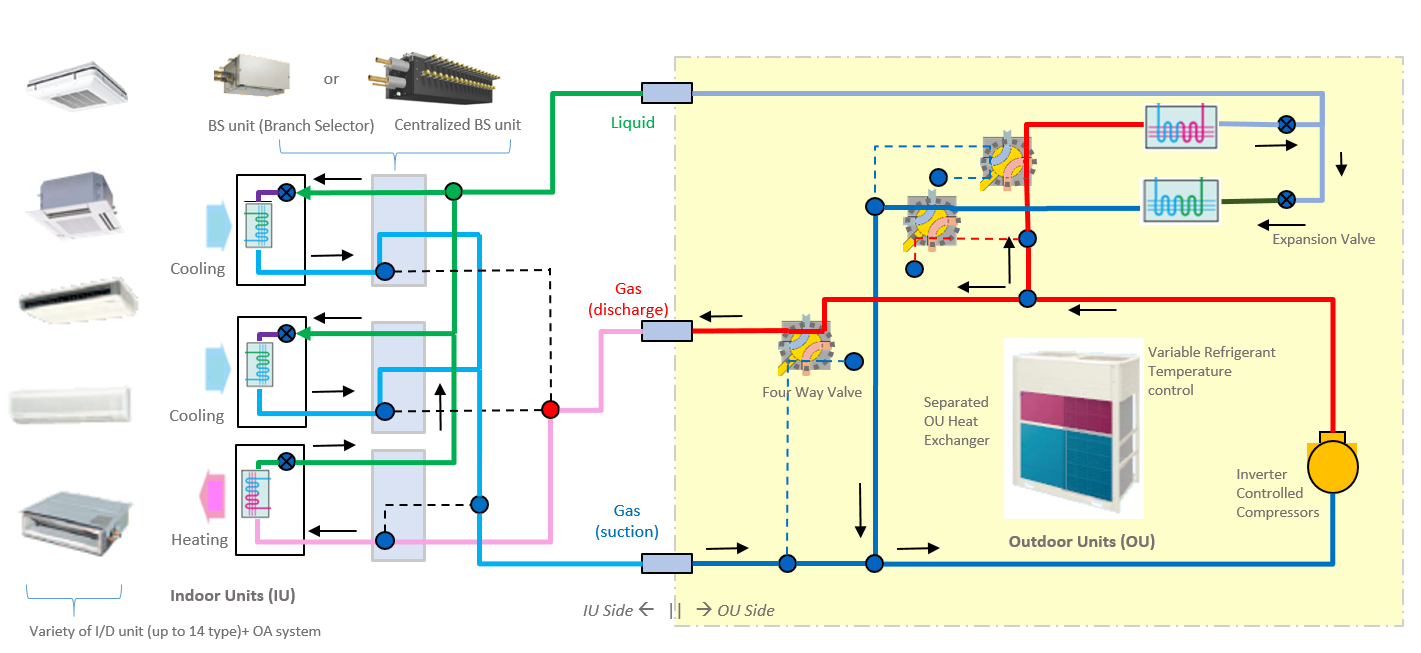
\includegraphics[width=0.95\textwidth, height=0.95\textheight, keepaspectratio=true]{media/VRF-HR-Chart-Schematic.png}
\caption{Schematic chart of a 3-pipe VRF-HR system \label{fig:VRF-HR-Chart-Schematic}}
\end{figure}


\paragraph{VRF-HR operational modes}\label{VRF-HR-operational-modes}

Depending on the indoor cooling/heating requirements and the outdoor unit operational states, the operations of the VRF-HR system can be categorized into six modes:

\begin{itemize}
  \item
  Mode 1: Cooling load only. No heating load. Both OU heat exchangers operate as condensers.
  \item
  Mode 2: Simultaneous heating and cooling. The sum of the zone cooling loads and compressor heat is much larger than the sum of the zone heating loads. Both OU heat exchangers operate as condensers.
  \item
  Mode 3: Simultaneous heating and cooling. The sum of the zone cooling loads and compressor heat is slightly larger than the sum of the zone heating loads. One OU heat exchanger operates as a condenser while the other as an evaporator.
  \item
  Mode 4: Simultaneous heating and cooling. The sum of the zone cooling loads and compressor heat is slightly smaller than the sum of the zone heating loads. One OU heat exchanger operates as a condenser while the other as an evaporator.
  \item
  Mode 5: Simultaneous heating and cooling. The sum of the zone cooling loads and compressor heat is much smaller than the sum of the zone heating loads. Both OU heat exchangers operate as evaporators.
  \item
  Mode 6: Heating load only. No cooling load. Both OU heat exchangers operate as evaporators.
\end{itemize}

\begin{figure}[hbtp] % figure VRF-HR-Chart-HeatBalance
\centering
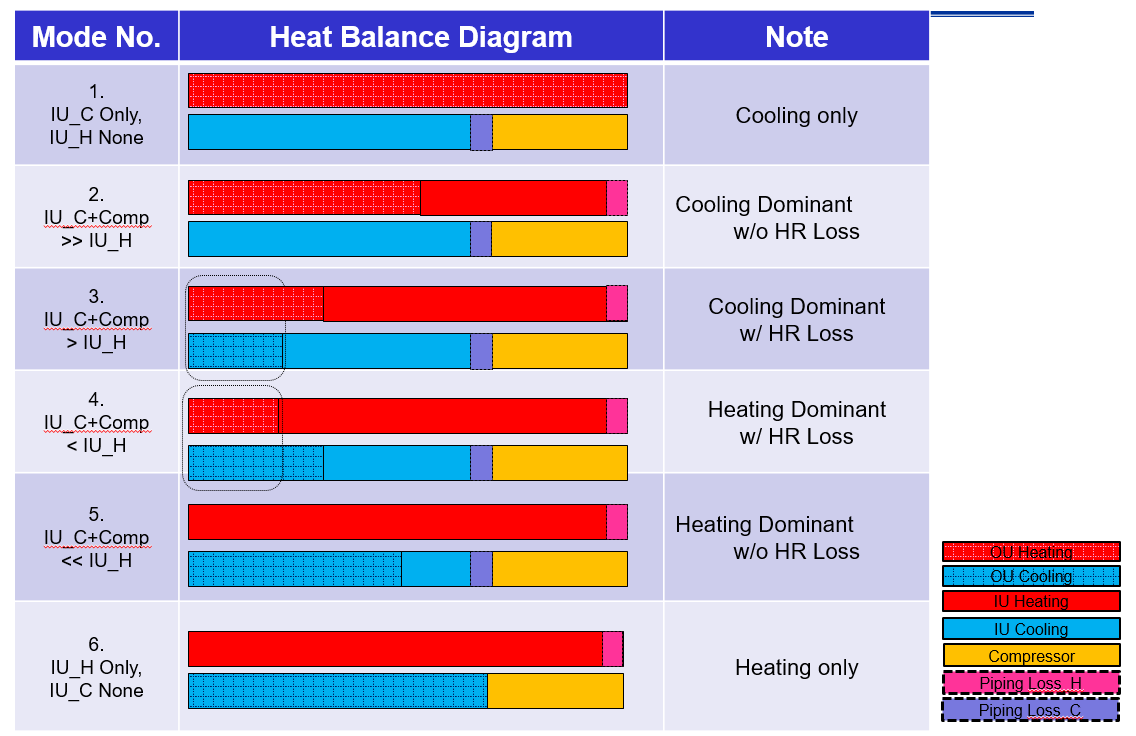
\includegraphics[width=0.95\textwidth, height=0.95\textheight, keepaspectratio=true]{media/VRF-HR-Chart-HeatBalance.png}
\caption{System-level Heat Balance Diagram for the Six VRF-HR Operational Modes \label{fig:VRF-HR-Chart-HeatBalance}}
\end{figure}

The system-level heat balance diagram for all the six operational modes are shown in Figure~\ref{fig:VRF-HR-Chart-HeatBalance}. Note that the heat recovery loss (HR loss) only exists in Mode 3 and Mode 4, in which the OU evaporator and condenser run simultaneously. In these modes, the following two items are at similar levels: (a) sum of IU heating loads and IU condenser side piping loss, and (b) sum of IU cooling loads, IU evaporator side piping loss and heat released by the compressor. Take Mode 3 for example, item (b) is higher than item (a), and therefore the system requires the operation of OU condenser to release the extra heat to ensure the system-level heat balance. However, the extra heat is at a relatively low level so that the system needs to release more heat than required via OU condenser and meanwhile runs OU evaporator to ensure the heat balance as well as system reliability. This leads to the presence of HR loss.


\paragraph{System operation at various modes}\label{System-operation-at-various-modes}

With the help of FWV and BS units, every operational mode has its own refrigerant piping connections to achieve different refrigerant flow directions, as shown in Figure~\ref{fig:VRF-HR-Chart-Piping}. This leads to different refrigerant operations and piping loss situations, as shown in the Pressure-Enthalpy Diagrams in Figure~\ref{fig:VRF-HR-Chart-EnthalpyPressure}.

Take Mode 3 for instance, the system utilizes one OU heat exchanger as an evaporator and the other as a condenser. The superheated refrigerant coming out of the compressor is divided into two parts. One part passes through the OU condenser within which the refrigerant is condensed and subcooled (segment 2-4’), while the other part passes through the IU condenser to satisfy the indoor heating requirements (segment 3-4). Note that before entering the IU condenser, the second part of the refrigerant flow passes through the main discharge gas pipe connecting the indoor and outdoor units, where the refrigerant pressure drop and heat loss occurs. This leads to extra heating load and a lower condensing temperature level at IU condenser than that at OU condenser. The two parts of refrigerant leaving condensers are then expanded through expansion valves following segment 4”-5/5’ and pass through the IU evaporator (segment 5-6) and OU evaporator (segment 5’-1’). Similarly to the refrigerant passing through the main discharge gas pipe, the refrigerant leaving IU evaporators passes through the main suction gas pipe where the refrigerant pressure drop and heat loss occurs (segment 6-1”). This leads to extra cooling load and a higher evaporating temperature level at IU evaporator than that at OU evaporator. Finally, the refrigerant flow leaving the OU evaporator and that leaving the main discharge gas pipe are combined (segment 1’/1”-1) and enter the compressors for the next cycle. In this regard, the system provides simultaneous heating and cooling to the indoor environment.

A number of operational parameters are controlled to ensure system heat balance and stable and reliable system operation, including evaporating temperature levels, condensing temperature levels, superheating and sub-cooling degrees, and the refrigerant flow rates at various components. The operational control logics for various modes are different and therefore particular algorithm needs to be designed for different operational modes in the new VRF-HR model.

\begin{figure}[hbtp] % figure VRF-HR-Chart-Piping
\centering
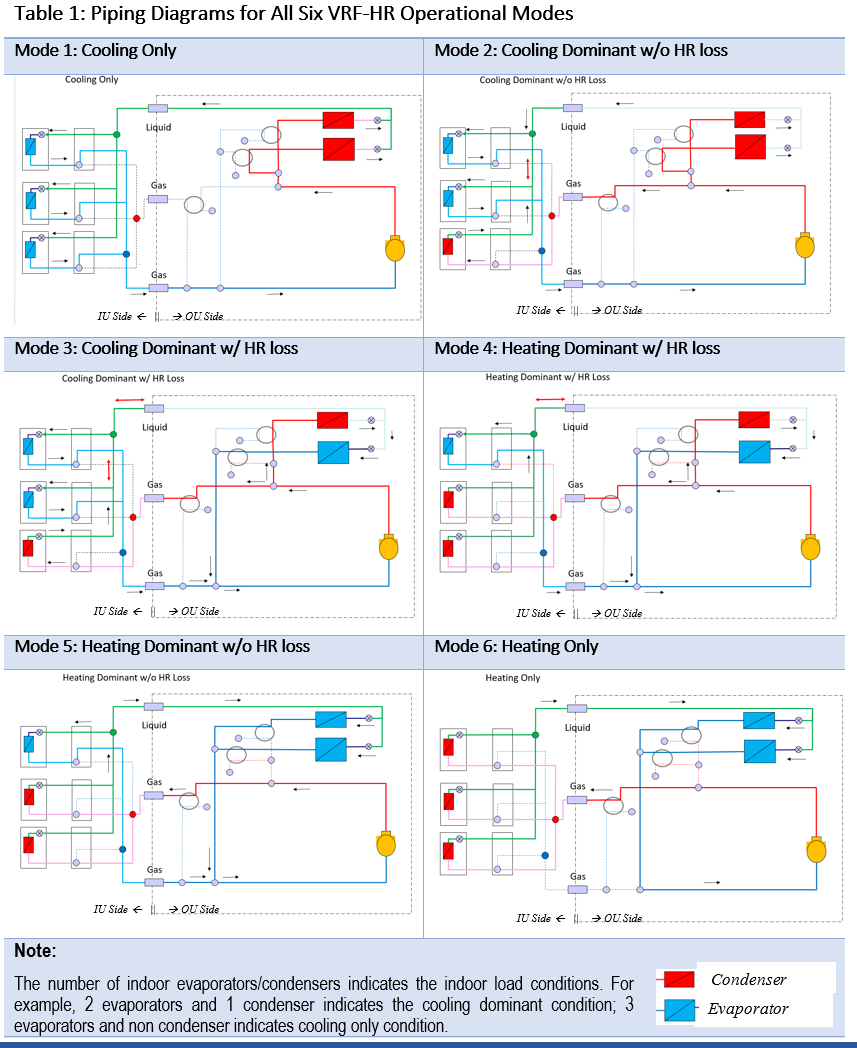
\includegraphics[width=0.95\textwidth, keepaspectratio=true]{media/VRF-HR-Chart-Piping.png}
\caption{Piping diagrams for the six VRF-HR operational modes \label{fig:VRF-HR-Chart-Piping}}
\end{figure}

\begin{figure}[hbtp] % figure VRF-HR-Chart-EnthalpyPressure
\centering
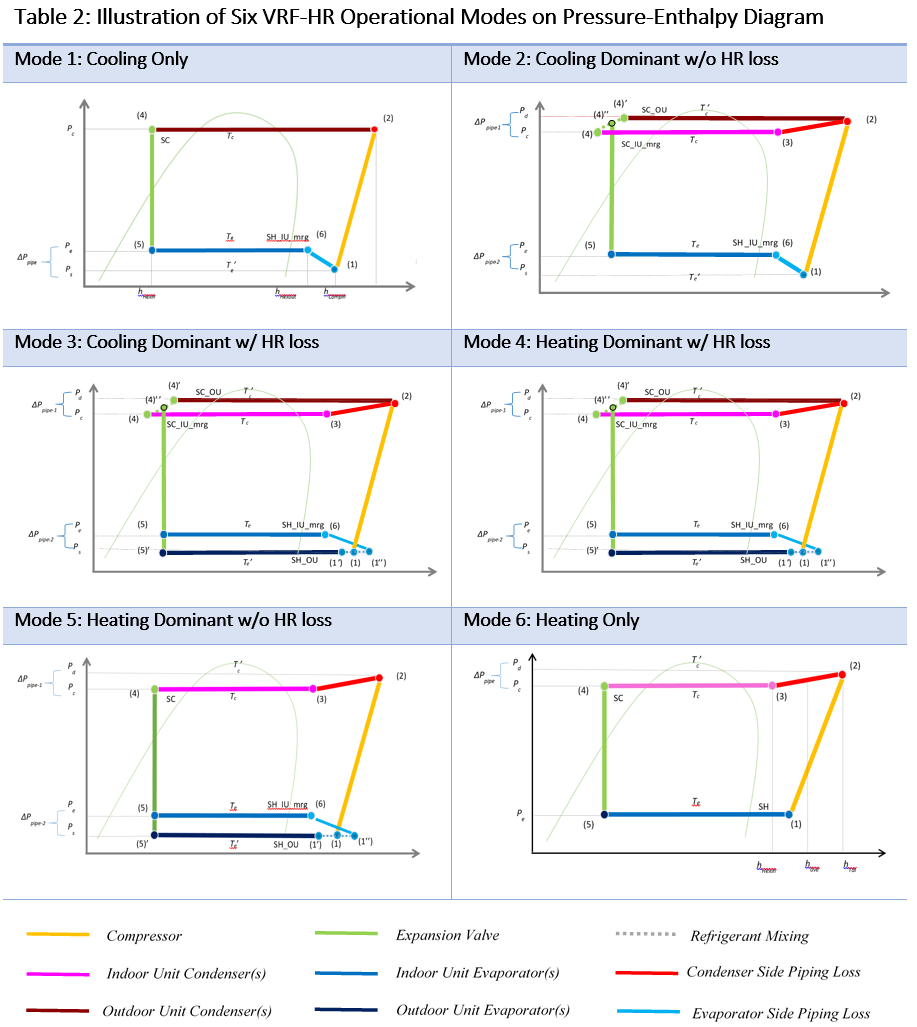
\includegraphics[width=0.95\textwidth, keepaspectratio=true]{media/VRF-HR-Chart-EnthalpyPressure.png}
\caption{Illustration of the six VRF-HR operational modes on Pressure-Enthalpy diagrams \label{fig:VRF-HR-Chart-EnthalpyPressure}}
\end{figure}

\subsubsection{Model Description}\label{vrf-heat-pump-model-description-2016-07-20-09-10}

The algorithm of the VRF-HR Cooling Only Mode and Heating Only Mode are the same as those in the VRF-HP Cooling Mode (Figure~\ref{fig:vrf-fluid-t-ctrl-3b}) and Heating Mode (Figure~\ref{fig:vrf-fluid-t-ctrl-3a}), respectively. The holistic logics of the VRF-HR Simultaneous Heating and Cooling Mode are illustrated in Figure~\ref{fig:VRF-HR-AlgorithmOverview-Mode2-5}. In general, the effective evaporating temperature and/or condensing temperature for the indoor units is first determined based on the load requirements and indoor unit configurations. Then the pressure and heat losses through the main pipe are calculated at the given operational conditions. After that, the effective condensing temperature and/or evaporating temperature of the outdoor unit is calculated, taking into account the piping loss. With the above calculations, the compressor speed can be determined using the performance curves describing the evaporative capacity of the system at specific condensing/evaporating temperature combinations at various compressor speeds. Finally, the compressor power at that speed is calculated and the total electric power consumption by the outdoor unit is obtained. Note that particular control logics are designed for various operational modes, and therefore lead to different refrigerant temperature adjustments. Also, note that a number of calculation steps are coupled together, for instance, the piping loss calculation and the system performance calculation. More specifically, the piping loss changes the operating conditions of the system, which may lead to a different control strategy and thus affect the amount of piping loss. This makes it difficult to obtain an analytical solution for a number of operational parameters (e.g., enthalpy of refrigerant entering the indoor unit), and therefore numerical iterations are employed to address this problem.

\begin{figure}[hbtp] % figure VRF-HR-AlgorithmOverview-Mode2-5
\centering
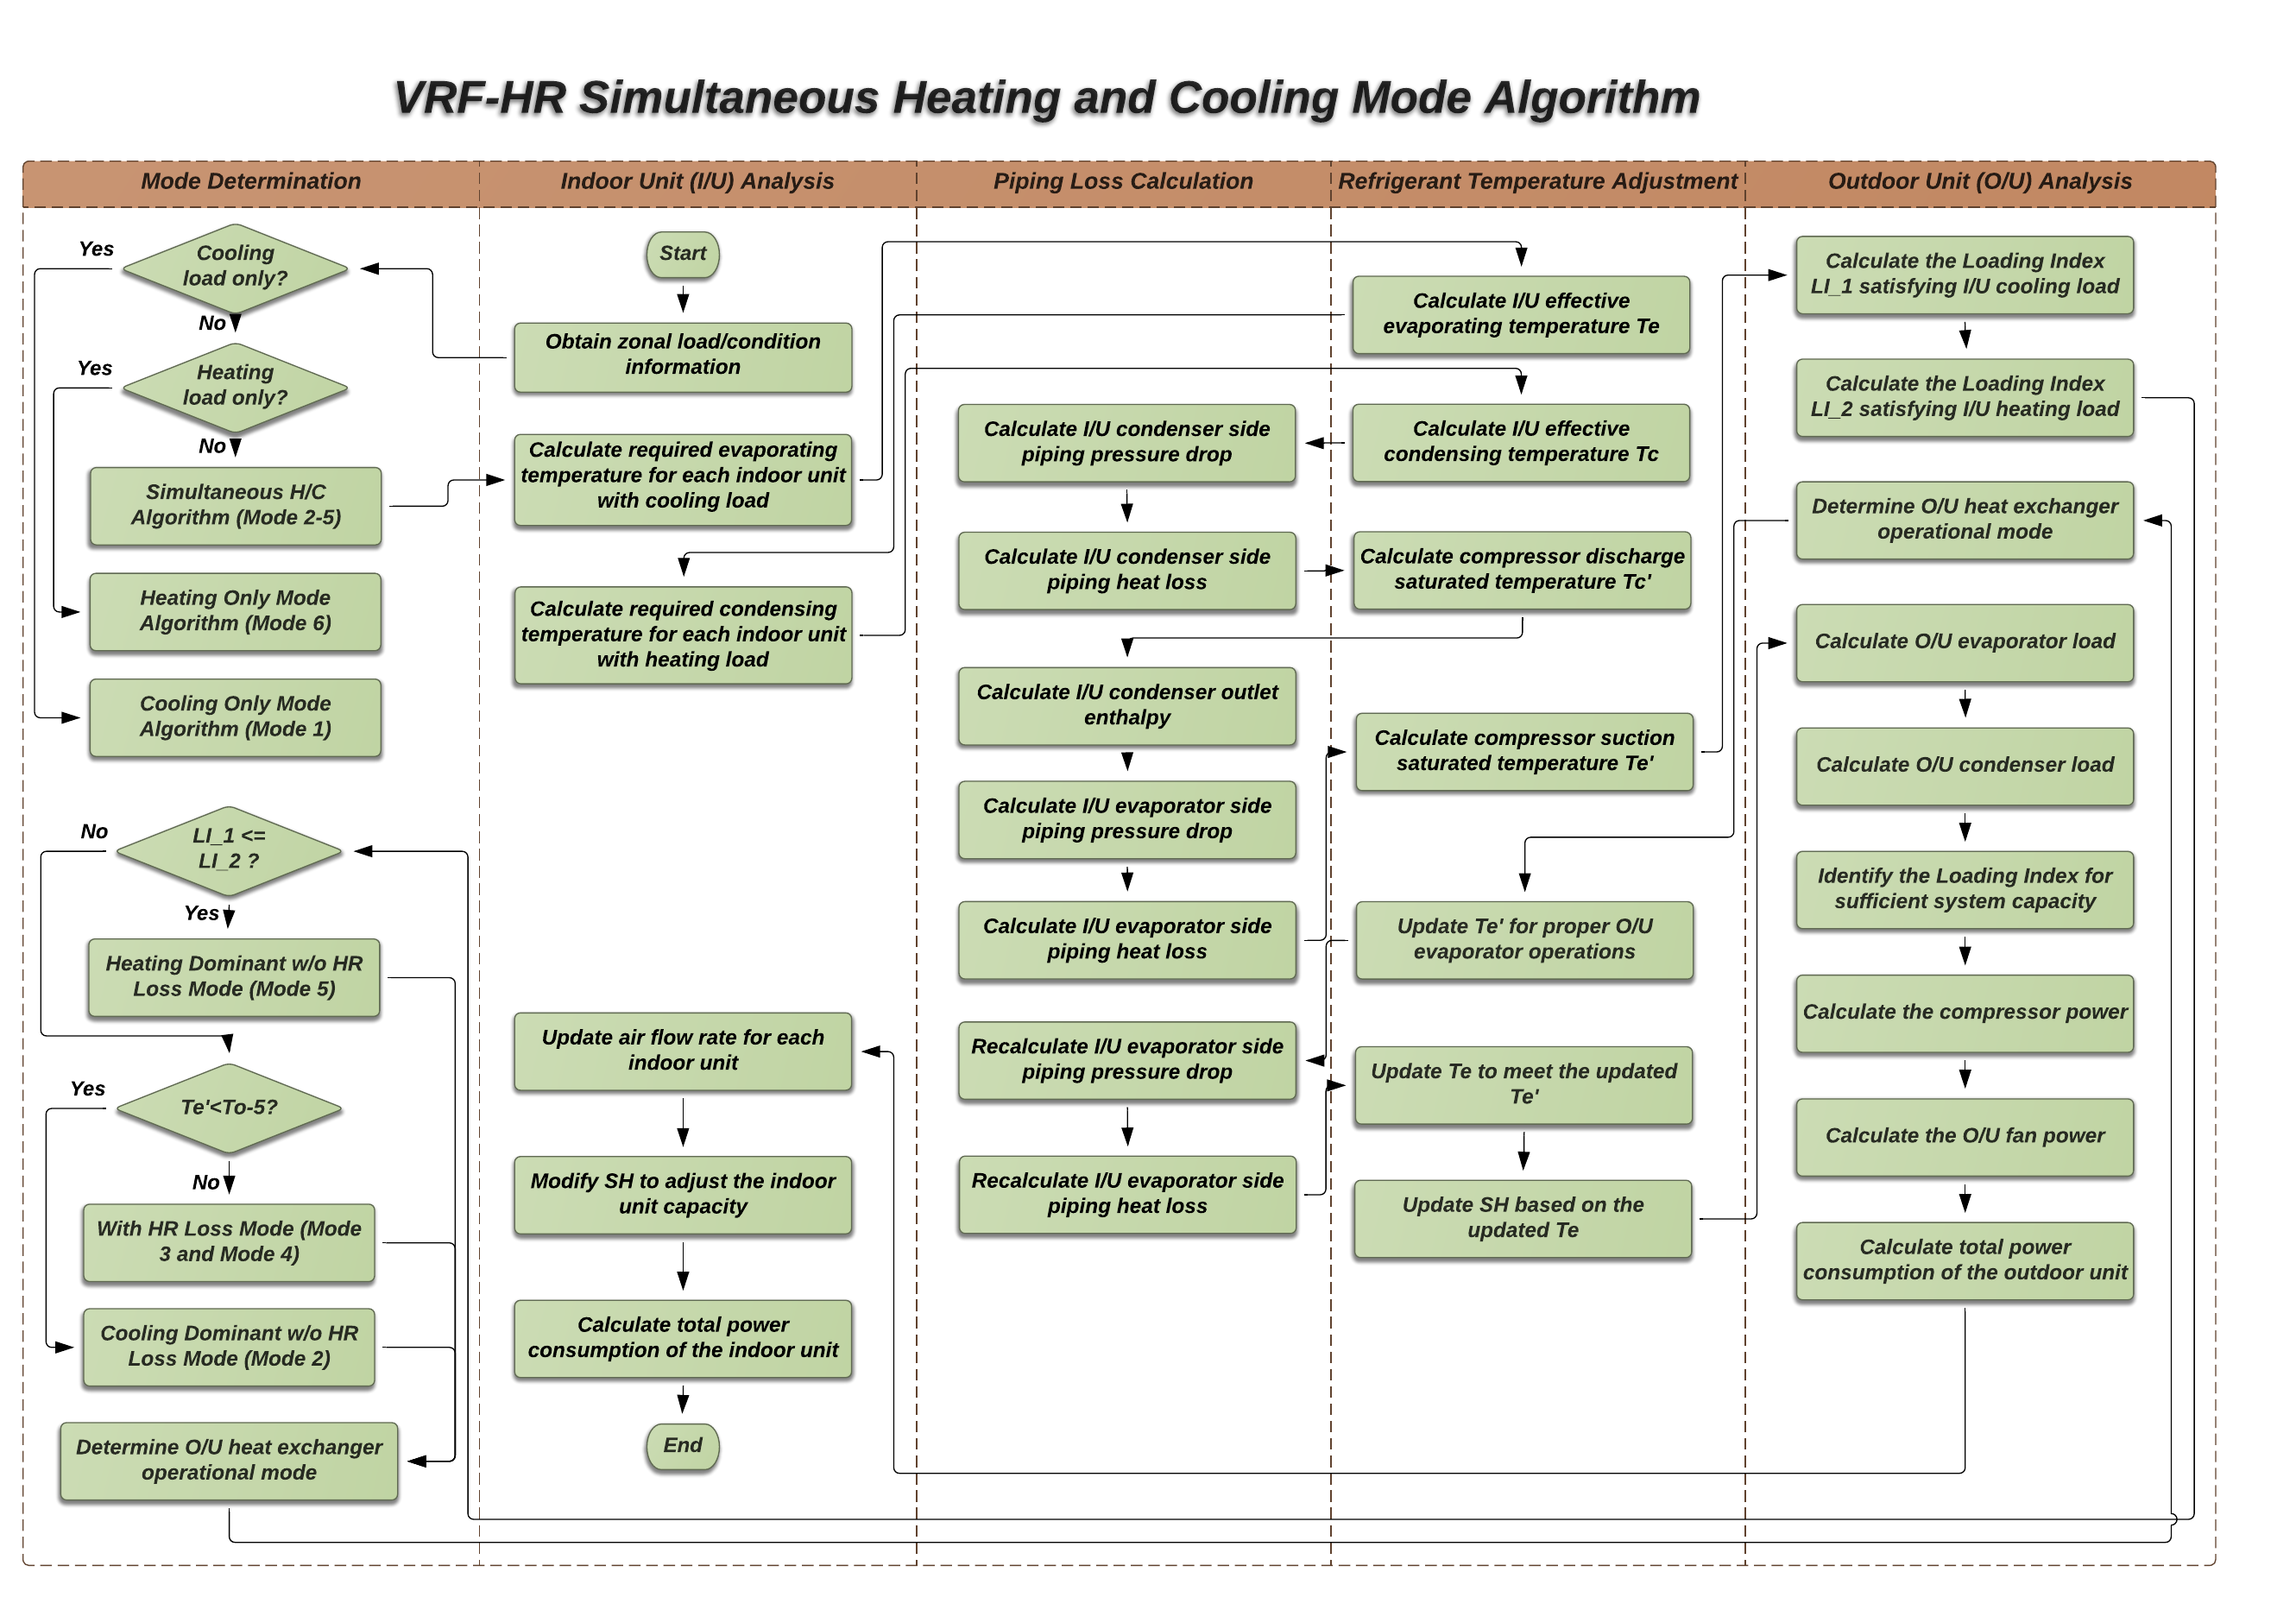
\includegraphics[width=0.9\textwidth, height=0.9\textheight, keepaspectratio=true]{media/VRF-HR-AlgorithmOverview-Mode2-5.png}
\caption{Schematic chart of the new VRF-HR algorithm: Simultaneous Heating and Cooling Mode \label{fig:VRF-HR-AlgorithmOverview-Mode2-5}}
\end{figure}

Detailed calculation procedures for the VRF-HR Simultaneous Heating and Cooling Mode are summarized as follows.

\textbf{Step 1: Obtaining zonal load/condition information}

The following information for each zone from the zone modules within EnergyPlus are obtained:

\begin{itemize}
  \item
    zone sensible loads $Q_{in, sensible}$
  \item
    zone total loads $Q_{in, total}$
  \item
    indoor air temperature $T_{in}$
  \item
    indoor air humidity ratio $W_{in}$
\end{itemize}

If there are only zone cooling loads and no zone heating loads, go to the VRF-HR Cooling Only Mode, the algorithms of which is the same as those for the VRF-HP Cooling Mode. If there are only zone heating loads and no zone cooling loads, go to the VRF-HR Heating Only Mode, the algorithms of which is the same as those for the VRF-HP Heating Mode. Otherwise, go to the VRF-HR Simultaneous Heating and Cooling Mode as described below.

\textbf{Step 2: Calculate IU required evaporating temperature and/or the condensing temperature}
Evaluate the required coil surface air temperature $T_{fs}$ and then the required evaporator refrigerant temperature $T_{e,req}$ for each indoor unit with cooling requirements. Likewise, evaluate the required condenser refrigerant temperature ${T_{c,req}}$ for each indoor unit with heating requirements.
(Refer to Step 1.2 in the VRF-FluidTCtrl-HP model for more details.)

\textbf{Step 3: Calculate IU effective evaporating temperature $T_e$ and/or the condensing temperature $T_c$}
There are two refrigerant temperature control strategies for the indoor unit: (1) \emph{ConstantTemp}, (2) \emph{VariableTemp}.

\begin{itemize}
  \item
    In the \emph{ConstantTemp} strategy, $T_e$ and $T_c$ are kept at constant values provided by the user.
  \item
    In the \emph{VariableTemp} strategy, $T_e$ and $T_c$ are determined using the required evaporating/condensing temperature calculated in Step 2.
\end{itemize}

(Refer to Step 1.3 in the VRF-FluidTCtrl-HP model for more details.)

\textbf{Step 4: IU condenser side piping loss calculations}

This section calculates the IU condenser side piping loss, which occurs at the High and Low Pressure Gas Pipe where the refrigerant flowing from the OU compressor outlets to the IU condensers. It includes both the refrigerant pressure drop $\Delta{P_{pipe}}$ and heat loss $Q_{pipe}$. Note that the change of compressor operational conditions may lead to different control strategies of the system, which in reverse affects the amount of piping loss. So the piping loss analysis and system performance analysis are coupled together. Numerical iterations are designed to address the coupling effect.

At this step, the compressor discharge saturated temperature $T'_c$ (i.e., saturated vapor temperature corresponding to compressor discharge pressure) can be obtained using the calculated refrigerant pressure drop $\Delta{P_{pipe}}$.

(Refer to Step 2h.1 in the VRF-FluidTCtrl-HP model for more details.)

\textbf{Step 5: IU evaporator side piping loss calculations}

This section calculates the IU evaporator side piping loss, which occurs at Suction Gas Pipe where the refrigerant flowing from the IU evaporators to the OU compressor inlets. Similarly to the IU condenser side piping loss, it includes both the refrigerant pressure drop $\Delta{P_{pipe}}$ and heat loss $Q_{pipe}$.

At this step, the compressor suction saturated temperature $T'_e$ (i.e., saturated vapor temperature corresponding to compressor suction pressure) can be obtained using the calculated refrigerant pressure drop $\Delta{P_{pipe}}$.

Note that one key input of the IU evaporator side piping loss calculations is the enthalpy of the refrigerant at IU evaporator inlets. It is assumed to be equal to the average enthalpy of the refrigerant at IU condenser outlets, which is obtained in the IU condenser side piping loss calculations.

(Refer to Step 2c.1 in the VRF-FluidTCtrl-HP model for more details.)

\textbf{Step 6: Determine the operational mode for simultaneous heating and cooling operations}

As noted earlier, simultaneous heating and cooling operations include the following modes:

\begin{itemize}
  \item
    Mode 2: Cooling dominant w/o HR loss
  \item
    Mode 3: Cooling dominant w/ HR loss
  \item
    Mode 4: Heating dominant w/ HR loss
  \item
    Mode 5: Heating dominant w/o HR loss
\end{itemize}

This section determines the operational mode based on the load requirements and operational conditions:

a. Calculate the Loading Index $LI_1$ satisfying IU cooling load (Refer to Step 2c.4 in the VRF-FluidTCtrl-HP model for more details.)

b. Calculate the Loading Index $LI_2$ satisfying IU heating load (Refer to Step 2h.4 in the VRF-FluidTCtrl-HP model for more details.)

c. If $LI_1$ $\leq$ $LI_2$, the system operates at Mode 5

d. If $LI_1$ $>$ $LI_2$ and $Te'$ $<$ $T_o$ - $T_{diff}$, the system operates at Mode 2
($T_o$: outdoor air dry-bulb temperature; $T_{diff}$: a constant value representing the difference between OU evaporating temperature and outdoor air temperature during simultaneous heating and cooling)

e. If $LI_1$ $>$ $LI_2$ and $Te'$ $\geq$  $T_o$ - $T_{diff}$, the system operates at Mode 3 or 4 (these two modes can be handled by one set of algorithms)

\textbf{Step 7: OU operation analysis at Mode 5}

\emph{\textbf{If $Te'$ $<$ $T_o$ - $T_{diff}$, perform the following procedures:}}

a. Select the compressor speed corresponding to $LI_2$

b. Calculate the compressor power corresponding to $LI_2$ and the previously obtained $T_c$ and $Te'$
(Refer to Step 2c.6 in the VRF-FluidTCtrl-HP model for more details.)

c. Calculate the evaporative capacity $Cap_{tot,evap}$ provided by the compressor at $LI_2$ and the previously obtained $T_c$ and $Te'$
(Refer to Step 2c.4 in the VRF-FluidTCtrl-HP model for more details.)

d. Calculate the OU evaporator load $Cap_{ou,evap}$ based on system-level heat balance

e. Obtain the OU fan flow rate $m_air_evap$ corresponding to $Cap_{ou,evap}$, and thus the fan power
(Refer to Step 2c.3 in the VRF-FluidTCtrl-HP model for more details.)

\emph{\textbf{If $Te'$ $\geq$  $T_o$ - $T_{diff}$, perform the following procedures:}}

a. Select the compressor speed corresponding to $LI_1$

b. Perform iterations between step b-i to identify the compressor Loading Index and power consumption.

c. Initialized compressor power $Ncomp_{ini}$

c.1 For the 1st iteration step, calculate $Ncomp$ = $f_{pow,comp}$( $T_c$, $T_o$ – 5, $LI_2$)

c.2 For the following iteration steps, update $Ncomp$ = ($Ncomp_{ini}$ + $Ncomp_{new}$)/2

d. Calculate the OU evaporator load $Cap_{ou,evap}$ based on system-level heat balance

e. Obtain the OU evaporating temperature $Te'$ level using $Cap_{ou,evap}$ and the rated air flow rate
(Refer to Step 2c.3 in the VRF-FluidTCtrl-HP model for more details.)

f. Update $T_e$ level and IU evaporator side piping loss, corresponding to $Te'$ update

g. Identify the compressor Loading Index $LI_{new}$ to provide sufficient evaporative capacity $Cap_{tot,evap}$ at updated $Te'$ level
(Refer to Step 2c.4 in the VRF-FluidTCtrl-HP model for more details.)

h. Calculate the compressor power $Ncomp_{new}$ corresponding to $LI_{new}$ and the updated $Te'$
(Refer to Step 2c.6 in the VRF-FluidTCtrl-HP model for more details.)

i. Compare $Ncomp_{new}$ and $Ncomp_{ini}$. Start a new round of iteration if the difference is greater than the tolerance.

\textbf{Step 8: OU operation analysis at Mode 2}

a. Select the compressor speed corresponding to $LI_1$

b. Calculate the compressor power corresponding to $LI_1$ and the previously obtained $T_c$ and $Te'$
(Refer to Step 2c.6 in the VRF-FluidTCtrl-HP model for more details.)

c. Calculate the evaporative capacity $Cap_{tot,evap}$ provided by the compressor at $LI_1$ and the previously obtained $T_c$ and $Te'$
(Refer to Step 2c.4 in the VRF-FluidTCtrl-HP model for more details.)

d. Calculate the OU condenser load $Cap_{ou,cond}$ based on system-level heat balance

e. Obtain the OU fan flow rate $m_{air,cond}$ corresponding to $Cap_{ou,cond}$, and thus the fan power

\textbf{Step 9: OU operation analysis at Mode 3 or 4}

a. Select the compressor speed corresponding to $LI_1$

b. Perform iterations between step b-e to identify the updated $Te'$ level within the range of $T_o$-5 and the original $Te'$.

c. Calculate the evaporative capacity $Cap_{tot,evap}$ provided by the compressor at $LI_1$ and the previously obtained $T_c$ and assumed $Te'$
(Refer to Step 2c.4 in the VRF-FluidTCtrl-HP model for more details.)

d. Calculate the OU evaporator load $Cap_{tot,evap}$ at assumed $Te'$ level and rated fan flow rate
(Refer to Step 2h.3 in the VRF-FluidTCtrl-HP model for more details.)

e. Perform iterations to identify the updated $Te'$ level to ensure the heat balance for the b. and c. calculations

f. Update $T_e$ level and IU evaporator side piping loss, corresponding to $Te'$ update

g. Calculate the compressor power corresponding to $LI_1$ and the updated $Te'$
(Refer to Step 2c.6 in the VRF-FluidTCtrl-HP model for more details.)

h. Calculate the OU condenser load $Cap_{ou,cond}$ based on system-level heat balance

i. Obtain the OU fan flow rate $m_{air,cond}$ corresponding to $Cap_{ou,cond}$, and thus the fan power

\textbf{Step 10: Modify IU operational parameters for capacity adjustments}

The air flow rate and $SH$/$SC$ value of each indoor unit can be manipulated to adjust the cooling/heating capacity.
(Refer to Step 3c and 3h in the VRF-FluidTCtrl-HP model for more details.)


\subsection{Zone Terminal Unit List}\label{zone-terminal-unit-list}

The zone terminal unit list identifies the terminal units that are connected to a single variable refrigerant flow heat pump. The zone terminal unit list is used exclusively in the variable refrigerant flow (VRF) heat pump object (ref: AirConditioner:VariableRefrigerantFlow) and VRF zone terminal units (ref: ZoneHVAC: TerminalUnit:VariableRefrigerantFlow). Up to 20 terminal units may be connected to a single VRF outdoor condensing unit. This list is extensible if additional indoor terminal units are required. The following figure shows the connection scheme between the zone terminal units, the zone terminal unit list, and finally the VRF AC system. The zone terminal units are connected to the zone through zone inlet and outlet zone nodes. Each zone terminal unit is entered in a list which represents all terminal units connected to a single VRF AC system. And finally, the zone terminal unit list name is entered in the corresponding VRF AC object.

\begin{figure}[hbtp] % fig 249
\centering
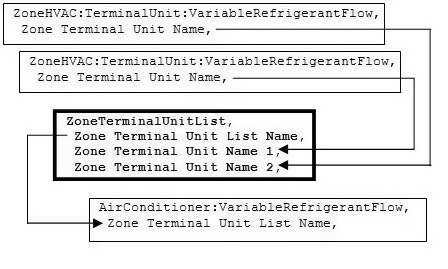
\includegraphics[width=0.9\textwidth, height=0.9\textheight, keepaspectratio=true]{media/image5454.png}
\caption{Zone Terminal List connections in EnergyPlus objects \protect \label{fig:zone-terminal-list-connections-in-energyplus}}
\end{figure}

\subsection{References}\label{references-051}

R. Raustad. A variable refrigerant flow heat pump computer model in EnergyPlus, ASHRAE Transactions (2013), 119 (1):1-9.

T. Hong, K. Sun, R. Zhang, R. Hinokuma, S. Kasahara, Y. Yura. Development and validation of a new variable refrigerant flow system model in EnergyPlus, Energy Build. 117 (2015): 399–411.

T. Hong, R. Zhang, K. Sun. Development, Validation and Performance Evaluation of VRF Heat Recovery Systems. LBNL Report, 2016.
